% Copyright (C) 2014-2020 by Thomas Auzinger <thomas@auzinger.name>

\documentclass[draft,final]{vutinfth} % Remove option 'final' to obtain debug information.

% Load packages to allow in- and output of non-ASCII characters.
\usepackage{lmodern}        % Use an extension of the original Computer Modern font to minimize the use of bitmapped letters.
\usepackage[T1]{fontenc}    % Determines font encoding of the output. Font packages have to be included before this line.
\usepackage[utf8]{inputenc} % Determines encoding of the input. All input files have to use UTF8 encoding.

% Extended LaTeX functionality is enables by including packages with \usepackage{...}.
\usepackage{amsmath}    % Extended typesetting of mathematical expression.
\usepackage{amssymb}    % Provides a multitude of mathematical symbols.
\usepackage{mathtools}  % Further extensions of mathematical typesetting.
\usepackage{microtype}  % Small-scale typographic enhancements.
\usepackage[inline]{enumitem} % User control over the layout of lists (itemize, enumerate, description).
\usepackage{multirow}   % Allows table elements to span several rows.
\usepackage{booktabs}   % Improves the typesettings of tables.
\usepackage{subcaption} % Allows the use of subfigures and enables their referencing.
\usepackage[ruled,linesnumbered,algochapter]{algorithm2e} % Enables the writing of pseudo code.
\usepackage[usenames,dvipsnames,table]{xcolor} % Allows the definition and use of colors. This package has to be included before tikz.
\usepackage{nag}       % Issues warnings when best practices in writing LaTeX documents are violated.
\usepackage{todonotes} % Provides tooltip-like todo notes.
\usepackage[backend=biber,style=trad-alpha,isbn=false,eprint=false,maxcitenames=3]{biblatex}
\usepackage{hyperref}  % Enables cross linking in the electronic document version. This package has to be included second to last.
\usepackage[acronym,toc]{glossaries} % Enables the generation of glossaries and lists fo acronyms. This package has to be included last.
\usepackage{siunitx}
\usepackage{float}
\usepackage{csquotes}

\addbibresource{references.bib}

% Define convenience functions to use the author name and the thesis title in the PDF document properties.
\newcommand{\authorname}{Tobias Eidelpes} % The author name without titles.
\newcommand{\thesistitle}{Plant Detection and State Classification with Machine Learning} % The title of the thesis. The English version should be used, if it exists.

% Set PDF document properties
\hypersetup
{
    pdfpagelayout   = TwoPageRight,           % How the document is shown in PDF viewers (optional).
    linkbordercolor = {Melon},                % The color of the borders of boxes around crosslinks (optional).
    pdfauthor       = {\authorname},          % The author's name in the document properties (optional).
    pdftitle        = {\thesistitle},         % The document's title in the document properties (optional).
    pdfsubject      = {Subject},              % The document's subject in the document properties (optional).
    pdfkeywords     = {Object Detection, Image Classification, Machine Learning, Embedded Programming} % The document's keywords in the document properties (optional).
}

\setpnumwidth{2.5em}        % Avoid overfull hboxes in the table of contents (see memoir manual).
\setsecnumdepth{subsection} % Enumerate subsections.

\nonzeroparskip             % Create space between paragraphs (optional).
\setlength{\parindent}{0pt} % Remove paragraph identation (optional).

\setcounter{tocdepth}{3}

\makeindex      % Use an optional index.
\makeglossaries % Use an optional glossary.
%\glstocfalse   % Remove the glossaries from the table of contents.

% Set persons with 4 arguments:
%  {title before name}{name}{title after name}{gender}
%  where both titles are optional (i.e. can be given as empty brackets {}).
\setauthor{}{\authorname}{BSc}{male}
\setadvisor{Ao.Univ.-Prof. Dr.}{Horst Eidenberger}{}{male}

\setregnumber{01527193}
\setdate{20}{02}{2023} % Set date with 3 arguments: {day}{month}{year}.
\settitle{\thesistitle}{Plant Detection and State Classification with Machine Learning} % Sets English and German version of the title (both can be English or German).

% Select the thesis type: bachelor / master / doctor / phd-school.
% Master:
\setthesis{master}
\setmasterdegree{dipl.} % dipl. / rer.nat. / rer.soc.oec. / master

% For bachelor and master:
\setcurriculum{Software Engineering \& Internet Computing}{Software Engineering \& Internet Computing} % Sets the English and German name of the curriculum.

\newacronym{xai}{XAI}{Explainable Artificial Intelligence}
\newacronym{grad-cam}{Grad-CAM}{Gradient-weighted Class Activation
  Mapping} \newacronym{cam}{CAM}{Class Activation Mapping}
\newacronym{oid}{OID}{Open Images Dataset} \newacronym{ap}{AP}{Average
  Precision} \newacronym{iou}{IOU}{Intersection over Union}
\newacronym{map}{mAP}{mean Average Precision}
\newacronym{resnet}{ResNet}{Residual Neural Network}
\newacronym{cnn}{CNN}{Convolutional Neural Network}
\newacronym{sgd}{SGD}{Stochastic Gradient Descent}
\newacronym{roc}{ROC}{Receiver Operating Characteristic}
\newacronym{auc}{AUC}{Area Under the Curve}
\newacronym{coco}{COCO}{Common Objects in Context}
\newacronym{voc}{VOC}{\textsc{PASCAL} Visual Object Classes}
\newacronym{sbc}{SBC}{single-board computer}
\newacronym{api}{API}{Application Programming Interface}
\newacronym{rest}{REST}{Representational State Transfer}
\newacronym{dl}{DL}{Deep Learning}
\newacronym{gpu}{GPU}{Graphics Processing Unit}
\newacronym{cpu}{CPU}{Central Processing Unit}
\newacronym{tpu}{TPU}{Tensor Processing Unit}
\newacronym{hog}{HOG}{Histogram of Oriented Gradients}
\newacronym{sift}{SIFT}{Scale-Invariant Feature Transform}
\newacronym{svm}{SVM}{Support Vector Machine}
\newacronym{dpm}{DPM}{Deformable Part-Based Model}
\newacronym{ai}{AI}{Artificial Intelligence}
\newacronym{mfcc}{MFCC}{Mel-frequency Cepstral Coefficient}
\newacronym{mlp}{MLP}{Multilayer Perceptron}
\newacronym{relu}{ReLU}{Rectified Linear Unit}
\newacronym{elu}{ELU}{Exponential Linear Unit}
\newacronym{silu}{SiLU}{Sigmoid Linear Unit}
\newacronym{mse}{MSE}{mean squared error}
\newacronym{ilsvrc}{ILSVRC}{ImageNet Large Scale Visual Recognition
Challenge}
\newacronym{lrn}{LRN}{Local Response Normalization}
\newacronym[plural=ROIs,longplural=Regions of Interest]{roi}{ROI}{Region of Interest}
\newacronym{spp}{SPP}{Spatial Pyramid Pooling}
\newacronym{rpn}{RPN}{Region Proposal Network}
\newacronym{fpn}{FPN}{Feature Pyramid Network}
\newacronym{yolo}{YOLO}{You Only Look Once}
\newacronym{ssd}{SSD}{Single Shot MultiBox Detector}
\newacronym{ann}{ANN}{Artificial Neural Network}
\newacronym{cuda}{CUDA}{Compute Unified Device Architecture}
\newacronym{rbf}{RBF}{Radial Basis Function}
\newacronym{mnist}{MNIST}{Modified National Institute of Standards and Technology}
\newacronym{aps-c}{APS-C}{Advanced Photo System type-C}
\newacronym{gcc}{GCC}{Green Canopy Cover}
\newacronym{gbdt}{GBDT}{Gradient Boosted Decision Tree}
\newacronym{dcnn}{DCNN}{Deep Convolutional Neural Networks}
\newacronym{k-nn}{k-NN}{k-Nearest Neighbors}
\newacronym{dt}{DT}{Decision Tree}
\newacronym{cart}{CART}{Classification and Regression Tree}
\newacronym{cnn-lstm}{CNN-LSTM}{CNN Long Short-Term Memory Network}
\newacronym{se}{SE}{Squeeze-Excitation}
\newacronym{bn}{BN}{Batch Normalization}
\newacronym{uav}{UAV}{Unmanned Aerial Vehicle}

\begin{document}

\frontmatter % Switches to roman numbering.
% The structure of the thesis has to conform to the guidelines at
%  https://informatics.tuwien.ac.at/study-services

\addtitlepage{naustrian} % German title page (not for dissertations at the PhD School).
\addtitlepage{english} % English title page.
\addstatementpage

\begin{danksagung*}
\todo{Ihr Text hier.}
\end{danksagung*}

\begin{acknowledgements*}
\todo{Enter your text here.}
\end{acknowledgements*}

\begin{kurzfassung}
\todo{Ihr Text hier.}
\end{kurzfassung}

\begin{abstract}
\todo{Enter your text here.}
\end{abstract}

% Select the language of the thesis, e.g., english or naustrian.
\selectlanguage{english}

% Add a table of contents (toc).
\tableofcontents % Starred version, i.e., \tableofcontents*, removes the self-entry.

% Switch to arabic numbering and start the enumeration of chapters in the table of content.
\mainmatter

\chapter{Introduction}
\label{chap:introduction}

Machine learning has seen an unprecedented rise in various research
fields during the last few years. Large-scale distributed computing
and advances in hardware manufacturing have allowed machine learning
models to become more sophisticated and complex. Multi-billion
parameter deep learning models show best-in-class performance in
\gls{nlp} \cite{brown2020}, fast object detection
\cite{bochkovskiy2020} and various classification tasks
\cite{zhong2022,ariss2022}. Agriculture is one of the areas which
profits substantially from the automation possible with machine
learning.

Large-scale as well as small local farmers are able to survey their
fields and gardens with drones or stationary cameras to determine soil
and plant condition as well as when to water or
fertilize~\cite{ramos-giraldo2020}. Machine learning models play an
important role in that process because they allow automated
decision-making in real time. While machine learning has been used in
large-scale agriculture, it is also a valuable tool for household
plants and gardens. By using machine learning to monitor and analyze
plant conditions, homeowners can optimize their plant care and ensure
their plants are healthy and thriving.

\section{Motivation and Problem Statement}
\label{sec:motivation}

The challenges to implement an automated system for plant surveying
are numerous. First, gathering data in the field requires a network of
sensors which are linked to a central server for processing. Since
communication between sensors is difficult without proper
infrastructure, there is a high demand for processing the data on the
sensor itself~\cite{mcenroe2022}. Second, differences in local soil,
plant and weather conditions require models to be optimized for these
diverse inputs. Centrally trained models often lose the nuances
present in the data because they have to provide actionable
information for a larger area~\cite{awad2019}. Third, specialized
methods such as hyper- or multispectral imaging in the field provide
fine-grained information about the object of interest but come with
substantial upfront costs and are of limited interest for gardeners.

To address all of the aforementioned problems, there is a need for an
installation which is deployable by homeowners, gathers data using
readily available hardware and performs computation on the device
without a connection to a central server. The device should be able to
visually determine whether the plants in its field of view need water
or not and output its recommendation. The recommendation should then
be used as a data point off of which homeowners can automatically
water their plants with an automated watering system.

The aim of this work is to develop a prototype which can be deployed
by gardeners to survey plants and recommend watering or not. To this
end, a machine learning model will be trained to first identify the
plants in the field of view and then to determine if the plants need
water or not. The model should be suitable for edge devices equipped
with a \gls{tpu} or \gls{gpu} but with otherwise limited processing
capabilities. Examples of such systems include Google's Coral
development board and the Nvidia Jetson series of~\glspl{sbc}. The
model should make use of state-of-the-art algorithms from either
classical machine learning or deep learning. The literature review
will yield an appropriate machine learning method. Furthermore, the
adaption of existing models (transfer learning) for object detection
to the domain of plant recognition may provide higher performance than
would otherwise be achievable within the time constraints.

The model will be deployed to the single-board computer and evaluated
using established and well-known metrics from the field of machine
learning. The evaluation will seek to answer the following questions:

\begin{enumerate}
\item \emph{How well does the model work in theory and how well in
    practice?}

  We will measure the performance of our model with common metrics
  such as accuracy, F-score, \gls{roc} curve, \gls{auc}, \gls{iou} and
  various \gls{map} measures. These measurements will allow
  comparisons between our model and existing models. We expect the
  plant detection part of the model to achieve high scores on the test
  dataset. However, the classification of plants into stressed and
  non-stressed will likely prove to be more difficult. The model is
  limited to physiological markers of water stress and thus will have
  difficulties with plants which do not overtly display such features.

  Even though models may work well in theory, some do not easily
  transfer to practical applications. It is, therefore, important to
  examine if the model is suited for productive use in the field. The
  evaluation will contain a discussion about the model's
  transferability because theoretical performance does not
  automatically guarantee real-world performance due to different
  environmental conditions.
\item \emph{What are possible reasons for it to work/not work?}

  Even if a model scores high on performance metrics, there might be a
  mismatch between how researchers think it achieves its goal and how
  it actually achieves its goal. The results have to be plausible and
  explainable with its inputs. Otherwise, there can be no confidence
  in the model's outputs. Conversely, if the model does not work,
  there must be a reason. We estimate that the curation of the dataset
  for the training and test phases will play a significant
  role. Explanations for model out- or underperformance are likely to
  be found in the structure and composition of the model's inputs.
\item \emph{What are possible improvements to the system in the
    future?}

  The previous two questions will yield the data for possible
  improvements to the model and/or our approach. With the decision to
  include a plant detection step at the start, we hope to create
  consistent conditions for the stress classification. A downside to
  this approach is that errors during detection can be propagated
  through the system and result in adverse effects to overall
  performance. Although we estimate this problem to be negligible,
  additional feedback regarding our approach in this way might offer
  insight into potential improvements. If the model does not work as
  well as expected, which changes to the approach will yield a better
  result? Similarly to the previous question, the answer will likely
  lie in the dataset. A heavy focus on dataset construction and
  curation will ensure satisfactory model performance.
\end{enumerate}

\section{Methodological Approach}
\label{sec:methods}

The methodological approach consists of the following steps:

\begin{enumerate}
\item \textbf{Literature Review}: The literature review informs the
  type of machine learning methods which are later applied during the
  implementation of the prototype.
\item \textbf{Dataset Curation}: After selecting the methods to use
  for the implementation, we have to create our own dataset or use
  existing ones, depending on availability.
\item \textbf{Model Training}: The selected models will be trained
  with the datasets curated in the previous step.
\item \textbf{Optimization}: The selected models will be optimized
  with respect to their parameters.
\item \textbf{Deployment to \gls{sbc}}: The software prototype will be
  deployed to the single-board computer.
\item \textbf{Evaluation}: The models will be evaluated extensively
  and compared to other state-of-the-art systems. During evaluation,
  the author seeks to provide a basis for answering the research
  questions.
\end{enumerate}

During the literature review, the search is centered around the terms
\emph{plant classification}, \emph{plant state classification},
\emph{plant detection}, \emph{water stress detection}, \emph{machine
learning agriculture}, \emph{crop machine learning} and \emph{remote
sensing}. These terms provide a solid basis for understanding the
state of the art in plant detection and stress classification. We will
use multiple search engines such as Google Scholar, Semantic Scholar,
the ACM Digital Library, and IEEE Xplore. It is common to only publish
research papers in preprint form in the data science and machine
learning fields. For this reason, we will also reference arXiv.org for
these papers. The work discovered in this way will also lead to
further insights about the type of models which are commonly used.

In order to find and select appropriate datasets to train the models
on, we will survey the existing big datasets for classes we can
use. Datasets such as the \gls{coco}~\cite{lin2015} and
\gls{voc}~\cite{everingham2010} contain the highly relevant class
\emph{Potted Plant}. By extracting only these classes from multiple
datasets and concatenating them together, it is possible to create one
unified dataset which only contains the classes necessary for training
the model.

The training of the models will happen in an environment where more
computational resources are available than what the~\gls{sbc}
offers. We will deploy the final model with the~\gls{api} to
the~\gls{sbc} after training and optimization. Furthermore, training
will happen in tandem with a continuous evaluation process. After
every iteration of the model, an evaluation run against the test set
determines if there has been an improvement in performance. The
results of the evaluation feed back into the parameter selection at
the beginning of each training phase. Small changes to the training
parameters, augmentations or structure of the model are followed by
another test phase. The iterative nature of the development of the
prototype increases the likelihood that the model's performance is not
only locally maximal but also as close as possible to the global
maximum.

In the final evaluation phase, we will measure the resulting model
against the test set and evaluate its performance with common
metrics. The aim is to first provide a solid basis of facts regarding
the model(s). Second, the results will be discussed in detail. Third,
we will cross-check the results with the hypotheses from
section~\ref{sec:motivation} and determine whether the aim of the work
has been met, and—if not—give reasons for the rejection of all or part
of the hypotheses.

Overall, the development of our application follows an evolutionary
pototyping process~\cite{davis1992,sears2007}. Instead of producing a
full-fledged product from the start, development happens iteratively
in phases. The main phases and their order for the prototype at hand
are: model selection, implementation, and evaluation. The results of
each phase—for example, which model has been selected—inform the
decisions which have to be made in the next phase (implementation). In
other words, every subsequent phase is dependent on the results of the
previous phase. All three phases, in turn, constitute one iteration
within the prototyping process. At the start of the next prototype,
the results of the previous iteration determine the path forward.

The decision to use an evolutionary prototyping process follows in
large part from the problem to be solved (as specified in
section~\ref{sec:motivation}). Since the critical requirements have
been established from the start, it is possible to build a solid
prototype from the beginning by implementing only those features which
are well-understood. The aim is to allow the developer to explore the
problem further so that additional requirements which arise during
development can be incorporated properly.

The prototyping process is embedded within the concepts of the
\emph{Scientific Method}. This thesis not only produces a prototype,
but also explores the problem of plant detection and classification
scientifically. Exploration of the problem requires making falsifiable
hypotheses (see section~\ref{sec:motivation}), gathering empirical
evidence (see section~\ref{sec:results}), and accepting or rejecting
the initial hypotheses (see section~\ref{sec:discussion}). Empirical
evidence is provided by measuring the model(s) against out-of-sample
test sets. This provides the necessary foundation for acceptance or
rejection of the hypotheses.

\section{Thesis Structure}
\label{sec:structure}

The first part of the thesis (chapter~\ref{chap:background}) contains
the theoretical basis of the models which we use for the
prototype. Chapter~\ref{chap:design} goes into detail about the
requirements for the prototype, the overall design and architecture of
the recognition and classification pipeline, and the structure and
unique properties of the selected
models. Chapter~\ref{chap:implementation} expands on how the datasets
are used during training as well as how the prototype publishes its
classification results. Chapter~\ref{chap:evaluation} shows the
results of the testing phases as well as the performance of the
aggregate model. Futhermore, the results are compared with the
expectations and it is discussed whether they are explainable in the
context of the task at hand as well as benchmark results from other
datasets (\gls{coco}~\cite{lin2015}). Chapter~\ref{chap:conclusion}
concludes the thesis with a summary and an outlook on possible
improvements and further research questions.

\chapter{Theoretical Background}
\label{chap:background}

Describe the contents of this chapter.

\begin{itemize}
\item Introduction to Object Detection, short ``history'' of methods,
  region-based vs. single-shot, YOLOv7 structure and successive
  improvements of previous versions. (8 pages)
\item Introduction to Image Classification, short ``history'' of
  methods, CNNs, problems with deeper network structures (vanishing
  gradients, computational cost), methods to alleviate these problems
  (alternative activation functions, normalization, residual
  connections, different kernel sizes). (10 pages)
\item Introduction into transfer learning, why do it and how can one
  do it? Compare fine-tuning just the last layers vs. fine-tuning all
  of them. What are the advantages/disadvantages of transfer learning?
  (2 pages)
\item Introduction to hyperparameter optimization. Which methods exist
  and what are their advantages/disadvantages? Discuss the ones used
  in this thesis in detail (random search and evolutionary
  optimization). (3 pages)
\item Related Work. Add more approaches and cross-reference the used
  networks with the theoretical sections on object detection and image
  classification. (6 pages)
\end{itemize}

Estimated 25 pages for this chapter.

\section{Machine Learning}
\label{sec:theory-ml}

The term machine learning was first used by \textcite{samuel1959} in
1959 in the context of teaching a machine how to play the game
Checkers. \textcite{mitchell1997a} defines learning in the context of
programs as:
\begin{quote}
  A computer program is said to \textbf{learn} from experience $E$
  with respect to some class of tasks $T$ and performance measure $P$,
  if its performance at tasks in $T$, as measured by $P$, improves
  with experience $E$. \cite[p.2]{mitchell1997a}
\end{quote}
In other words, if the aim is to learn to win at a game, the
performance measure $P$ is defined as the ability to win at that
game. The tasks in $T$ are playing the game multiple times, and the
experience $E$ is gained by letting the program play the game against
itself.

Machine learning is thought to be a sub-field of \gls{ai}. \gls{ai} a
more general term for the scientific endeavour of creating things
which possess the kind of intelligence we humans have. Since those
things will not have been created \emph{naturally}, their intelligence
is termed \emph{artificial}. Within the field of \gls{ai} there have
been other approaches than what is commonly referred to as machine
learning today.

A major area of interest in the 1980s was the development of
\emph{expert systems}. These systems try to approach problem solving
as a rational decision-making process. Starting from a knowledge base,
which contains facts and rules about the world and the problem to be
solved, the expert system applies an inference engine to arrive at a
conclusion. An advantage of these systems is that they can often
explain how they came to a particular conclusion, allowing humans to
verify and judge the inference process. This kind of explainability is
missing in the neural network based approaches of today. However, an
expert system needs a significant base of facts and rules to be able
to do any meaningful inference. Outside of specialized domains such as
medical diagnosis, expert systems have always failed at commonsense
reasoning.

Machine learning can be broadly divided into two distinct approaches:
\emph{supervised} and \emph{unsupervised}. Supervised learning
describes a process where the algorithm receives input values as well
as their corresponding output values and tries to learn the function
which maps inputs to outputs. This is called supervised learning
because the model knows a target to map to. In unsupervised learning,
in contrast, algorithms do not have access to labeled data or output
values and therefore have to find patterns in the underlying
inputs. There can be mixed approaches as in \emph{semi-supervised}
learning where a model receives a small amount of labeled data as an
aid to better extract the patterns in the unlabeled data. Which type
of learning to apply depends heavily on the problem at hand. Tasks
such as image classification and speech recognition are good
candidates for supervised learning. If a model is required to
\emph{generate} speech, text or images, an unsupervised approach makes
more sense. We will go into detail about the general approach in
supervised learning because it is used throughout this thesis when
training the models.

\subsection{Supervised Learning}
\label{ssec:theory-sl}

The overall steps when training a model with labeled data are as
follows:

\begin{enumerate}
\item Determine which type of problem is to be solved and select
  adequate training samples.
\item Gather enough training samples and obtain their corresponding
  targets (labels). This stage usually requires humans to create a
  body of ground truth with which the model can compare itself.
\item Select the type of representation of the inputs which is fed to
  the model. The representation heavily relies on the amount of data
  which the model can process in a reasonable amount of time. For
  speech recognition, for example, raw waveforms are rarely fed to any
  classifier. Instead, humans have to select a less granular and more
  meaningful representation of the waveforms such as
  \glspl{mfcc}. Selecting the representation to feed to the model is
  also referred to as \emph{feature selection} or \emph{feature
  engineering}.
\item Select the structure of the model or algorithm and the learning
  function. Depending on the problem, possible choices are
  \glspl{svm}, \glspl{cnn} and many more.
\item Train the model on the training set.
\item Validate the results on out-of-sample data by computing common
  metrics and comparing the results to other approaches.
\item Optionally go back to 4. to select different algorithms or to
  train the model with different parameters or adjusted training
  sets. Depending on the results, one can also employ computational
  methods such as hyperparameter optimization to find a better
  combination of model parameters.
\end{enumerate}

These steps are generally the same for every type of supervised or
semi-supervised machine learning approach. The implementation for
solving a particular problem differs depending on the type of problem,
how much data is available, how much can reasonably be labeled and any
other special requirements such as favoring speed over accuracy.

\subsection{Artificial Neural Networks}
\label{ssec:theory-nn}

Artificial neural networks are the building blocks of most
state-of-the-art models in use today. The computer sciences have
adopted the term from biology where it defines the complex structure
in the human brain which allows us to experience and interact with the
world around us. A neural network is necessarily composed of neurons
which act as gatekeepers for the signals they receive. Depending on
the inputs—electrochemical impulses, numbers, or other—the neuron
\emph{excites} and produces an output value if the right conditions
are met. This output value travels via connections to other neurons
and acts as an input on their side. Each neuron and connection between
the neurons has an associated weight which changes when the network
learns. The weights increase or decrease the signal from the
neuron. The neuron itself only passes a signal on to its output
connections if the conditions of its \emph{activation function} have
been met. This is typically a non-linear function. Multiple neurons
are usually grouped together to form a \emph{layer} within the
network. Multiple layers are stacked one after the other with
connections in-between to form a neural network. Layers between the
input and output layers are commonly referred to as \emph{hidden
layers}. Figure~\ref{fig:neural-network} shows the structure of a
three-layer fully-connected artificial neural network.

\begin{figure}
  \centering
  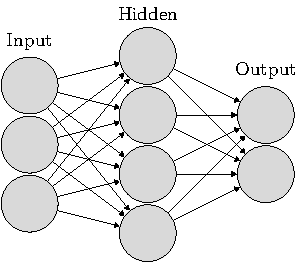
\includegraphics[width=0.5\textwidth]{graphics/neural-network/neural-network.pdf}
  \caption[Structure of an artificial neural network]{Structure of an
    artificial neural network. Information travels from left to right
    through the network using neurons and the connections between
    them.}
  \label{fig:neural-network}
\end{figure}

The earliest attempts at describing learning machines were by
\textcite{mcculloch1943} with the idea of the \emph{perceptron}. This
idea was implemented in a more general sense by
\textcite{rosenblatt1957,rosenblatt1962} as a physical machine. At its
core, the perceptron is the simplest artifical neural network with
only one neuron in the center. The neuron takes all its inputs,
aggregates them with a weighted sum and outputs 1 if the result is
above some threshold $\theta$ and 0 if it is not (see
equation~\ref{eq:perceptron}). This function is called the
\emph{activation function} of a perceptron. A perceptron is a type of
binary classifier which can only classify linearly separable
variables.

\begin{equation}
  \label{eq:perceptron}
  y =
  \begin{cases}
    1\;\mathrm{if}\;\sum_{i=1}^{n}w_i\cdot x_i\geq\theta \\
    0\;\mathrm{if}\;\sum_{i=1}^{n}w_i\cdot x_i<\theta
  \end{cases}
\end{equation}

Due to the inherent limitations of perceptrons to only be able to
classify linearly separable data, \glspl{mlp} are the bedrock of
modern artifical neural networks. By adding an input layer, a hidden
layer, and an output layer as well as requiring the activation
function of each neuron to be non-linear, a \gls{mlp} can classify
also non-linear data. Every neuron in each layer is fully connected to
all of the neurons in the next layer and it is the most
straightforward case of a feedforward
network. Figure~\ref{fig:neural-network} shows the skeleton of a
\gls{mlp}.

There are two types of artifical neural networks: feedforward and
recurrent networks. Their names refer to the way information flows
through the network. In a feedforward network, the information enters
the network and flows only uni-directionally to the output nodes. In a
recurrent network, information can also feed back into previous
nodes. Which network is best used depends on the task at
hand. Recurrent networks are usually necessary when \emph{context} is
needed. For example, if the underlying data to classify is a time
series, individual data points have some relation to the previous and
next points in the series. Maintaining a bit of state is beneficial
because networks should be able to capture these
dependencies. However, having additional functionality for feeding
information back into previous neurons and layers comes with increased
complexity. A feedforward network, as depicted in
Figure~\ref{fig:neural-network}, represents a simpler structure.

\subsection{Activation Functions}
\label{ssec:theory-activation-functions}

Activation functions are the functions \emph{inside} each neuron which
receive inputs and produce an output value. The nature of these
functions is that they need a certain amount of \emph{excitation} from
the inputs before they produce an output, hence the name
\emph{activation function}. Activation functions are either linear or
non-linear. Linear functions are limited in their capabilities because
they cannot approximate certain functions. For example, a perceptron,
which uses a linear activation function, cannot approximate the XOR
function \cite{minsky2017}. Non-linear functions, however, are a
requirement for neural networks to become \emph{universal
approximators} \cite{hornik1989}. We will introduce several activation
functions which are used in the field of machine learning in the
following sections. There exist many more than can be discussed within
the scope of this thesis. However, the selection should give an
overview of the most used and influential ones in the author's
opinion.

\subsubsection{Identity}
\label{sssec:theory-identity}

The simplest activation function is the identity function. It is defined as

\begin{equation}
  \label{eq:identity}
  g(x) = x
\end{equation}

If all layers in an artificial neural network use the identity
activation function, the network is equivalent to a single-layer
structure. The identity function is often used for layers which do not
need an activation function per se, but require one to uphold
consistency with the rest of the network structure.

\subsubsection{Heaviside Step}
\label{sssec:theory-heaviside}

The Heaviside step function, also known as the unit step function, is
a mathematical function that is commonly used in control theory and
signal processing to represent a signal that switches on at a
specified time and stays on. The function is named after Oliver
Heaviside, who introduced it in the late 19th century. It is defined
as

\begin{equation}
  \label{eq:heaviside}
  H(x) = 
  \begin{cases}
    1, x\geq 0 \\
    0, x < 0
  \end{cases}.
\end{equation}

In engineering applications, the Heaviside step function is used to
describe functions whose values change abruptly at specified values of
time $t$. We have already mentioned the Heaviside step function in
section~\ref{ssec:theory-nn} when introducing the perceptron. It can
only classify linearly separable variables when used in a neural
network and is, therefore, not suitable for complex intra-data
relationships. A major downside to using the Heaviside step function
is that it is not differentiable at $x = 0$ and has a $0$ derivative
elsewhere. These properties make it unsuitable for use with gradient
descent during back-propagation (section
\ref{ssec:theory-back-propagation}).

\subsubsection{Sigmoid}
\label{sssec:theory-sigmoid}

The sigmoid activation function is one of the most important functions
to introduce non-linearity into the outputs of a neuron. It is a
special case of a logistic function and used synonymously with
logistic function in machine learning. It is defined as

\begin{equation}
  \label{eq:sigmoid}
  \sigma(x) = \frac{1}{1 + e^{-x}}
\end{equation}

It has a characteristic S-shaped curve, mapping each input value to a
number between $0$ and $1$, regardless of input size. This
\emph{squashing} property is particularly desirable for binary
classification problems because the outputs can be interpreted as
probabilities. Additionally to the squashing propery, it is also a
saturating function because large values map to $1$ and very small
values to $0$. If a learning algorithm has to update the weights in
the network, saturated neurons are very inefficient and difficult to
process because the outputs do not provide valuable information. In
contrast to the Heaviside step function
(section~\ref{sssec:theory-heaviside}), it is differentiable which
allows it to be used with gradient descent optimization
algorithms. Unfortunately, the sigmoid function exacerbates the
vanishing gradient problem, which makes it unsuitable for training
deep neural networks.

\subsubsection{Rectified Linear Unit}
\label{sssec:theory-relu}

The \gls{relu} function is defined as

\begin{equation}
  \label{eq:relu}
  f(x) = \max(0, x) =
  \begin{cases}
    x, x > 0 \\
    0, x \leq 0
  \end{cases}
\end{equation}

which means that it returns the input value if it is positive, and
returns zero if it is negative. It was first introduced by
\textcite{fukushima1969} in a modified form to construct a visual
feature extractor. The \gls{relu} function is nearly linear, and it
thus preserves many of the properties that make linear models easy to
optimize with gradient-based methods \cite{goodfellow2016}. In
contrast to the sigmoid activation function, the \gls{relu} function
partially mitigates the vanishing gradient problem and is therefore
suitable for training deep neural networks. Furthermore, the
\gls{relu} function is easier to calculate than sigmoid functions
which allows networks to be trained more quickly. Even though it is
not differentiable at $0$, it is differentiable everywhere else and
often used with gradient descent during optimization.

The \gls{relu} function suffers from the dying \gls{relu} problem,
which can cause some neurons to become inactive. Large gradients,
which are passed back through the network to update the weights, are
typically the source of this. If many neurons are pushed into this
state, the model's capability of learning new patterns is
diminished. To address this problem, there are two possibilities. One
solution is to make sure that the learning rate is not set too high,
which reduces the problem but does not fully remove it. Another
solution is to use one of the several variants of the ReLU function
such as leaky \gls{relu}, \gls{elu}, and \gls{silu}.

In recent years, the \gls{relu} function has become the most popular
activation function for deep neural networks and is recommended as the
default activation function in modern neural networks
\cite{goodfellow2016}. Despite its limitations, the \gls{relu}
function has become an essential tool for deep learning practitioners
and has contributed to the success of many state-of-the-art models in
computer vision, natural language processing, and other domains.

\subsubsection{Softmax}
\label{sssec:theory-softmax}

The softmax activation function is often used as the last activation
function of a neural network to normalize the output of a network to a
probability distribution over predicted output classes. It takes a
vector of numbers, known as logits, and scales them into
probabilities. The output of the softmax function is a vector with
probabilities of each possible outcome, and the probabilities in the
vector sum to one for all possible outcomes or classes. In
mathematical terms, the function is defined as

\begin{equation}
  \label{eq:softmax}
  \sigma(\vec{z})_{i} = \frac{e^{z_i}}{\sum_{j=1}^Ke^{z_j}}i\ \mathrm{for}\ i = 1,\dots,K\ \mathrm{and}\ \vec{z} = (z_1,\dots,z_K)\in\mathbb{R}^K
\end{equation}

where the standard exponential function is applied to each value in
the vector $\vec{z}$ and the result is normalized with the sum of the
exponentials.

\subsection{Loss Function}
\label{ssec:theory-loss-function}

Loss functions play a fundamental role in machine learning, as they
are used to evaluate the performance of a model and guide its
training. The choice of loss function can significantly impact the
accuracy and generalization of the model. There are various types of
loss functions, each with its strengths and weaknesses, and the
appropriate choice depends on the specific problem being addressed.

From the definition of a learning program from
section~\ref{sec:theory-ml}, loss functions constitute the performance
measure $P$ against which the results of the learning program are
measured. Only by minimizing the error obtained from the loss function
and updating the weights within the network is it possible to gain
experience $E$ at carrying out a task $T$. How the weights are updated
depends on the algorithm which is used during the \emph{backward pass}
to minimize the error. This type of procedure is referred to as
\emph{back-propagation} (see
section~\ref{ssec:theory-back-propagation}).

One common type of loss function is the \gls{mse} which is widely used
in regression problems. The \gls{mse} is a popular choice because it
is easy to compute and has a closed-form solution, making it efficient
to optimize. It does have some limitations, however. For instance, it
is sensitive to outliers, and it may not be appropriate for problems
with non-normal distributions. \gls{mse} measures the average squared
difference between predicted and actual values. It is calculated with

\begin{equation}
  \label{eq:mse}
  \mathrm{MSE_{test}} = \frac{1}{m}\sum_i(\hat{y}^{(\mathrm{test})} - y^{(\mathrm{test})})_i^2
\end{equation}

where $\hat{y}^{(\mathrm{test})}$ contains the predictions of the
model on the test set and $y^{(\mathrm{test})}$ refers to the target
labels \cite{goodfellow2016}. It follows that, if
$\hat{y}^{(\mathrm{test})} = y^{(\mathrm{test})}$, the error is $0$
and the model has produced a perfect prediction.

We cannot, however, take the results of the error on the test set to
update the weights during training because the test set must always
contain only samples which the model has not seen before. If the model
is trained to minimize the \gls{mse} on the test set and then
evaluated against the same set, the results will be how well the model
fits to the test set and not how well it generalizes. The goal,
therefore, is to minimize the error on the training set and to compare
the results against an evaluation on the test set. If the model
achieves very low error rates on the training set but not on the test
set, it is likely that the model is suffering from
\emph{overfitting}. Conversely, if the model does not achieve low
error rates on the training set, it is likely that the model is
suffering from \emph{underfitting}.

\textcite{goodfellow2016} writes on \gls{mse}: ``\gls{mse} was popular
in the 1980s and 1990s but was gradually replaced by cross-entropy
losses and the principle of maximum likelihood as ideas spread between
the statistics community and the machine learning
community''~\cite[p.222]{goodfellow2016}. Cross-entropy measures the
difference in information between two distinct probability
distributions. Specifically, it gives a number on the average total
amount of bits needed to represent a message or event from the first
probability distribution in the second probability distribution. If
there is the case of binary random variables, i.e. only two classes to
classify exist, the measure is called binary
cross-entropy. Cross-entropy loss is known to outperform \gls{mse} for
classification tasks and allows the model to be trained
faster~\cite{simard2003}.

\subsection{Back-Propagation}
\label{ssec:theory-back-propagation}

So far, information only flows forward through the network whenever a
prediction for a particular input should be made. In order for a
neural network to learn, information about the computed loss has to
flow backward through the network. Only then can the weights at the
individual neurons be updated. This type of information flow is termed
\emph{back-propagation} \cite{rumelhart1986}. Back-propagation
computes the gradient of a loss function with respect to the weights
of a network for an input-output pair. The algorithm computes the
gradient iteratively starting from the last layer and works its way
backward through the network until it reaches the first layer.

Strictly speaking, back-propagation only computes the gradient, but
does not determine how the gradient is used to learn the new
weights. Once the back-propagation algorithm has computed the
gradient, that gradient is passed to an algorithm which finds a local
minimum of it. This step is usually performed by some variant of
gradient descent \cite{cauchy1847}.

\section{Object Detection}
\label{sec:background-detection}

From facial detection to fully automated driving—object detection
provides the basis for a wide variety of tasks within the computer
vision world. While most implementations in the 1990s and early 2000s
relied on cumbersome manual feature extraction, current methods almost
exclusively leverage a deep learning based approach. This chapter
gives an introduction to object detection, explains common problems
researchers have faced and how they have been solved, and discusses
the two main approaches to object detection via deep learning.

\subsection{Traditional Methods}
\label{ssec:obj-traditional}

Before the advent of powerful \glspl{gpu}, object detection was
commonly done by manually extracting features from images and passing
these features on to a classical machine learning algorithm. Early
methods were generally far from being able to detect objects in real
time.

\subsubsection{Viola-Jones Detector}
\label{sssec:obj-viola-jones}

The first milestone was the face detector by
~\textcite{viola2001,viola2001} which is able to perform face
recognition on $384$ by $288$ pixel (grayscale) images with
\qty{15}{fps} on a \qty{700}{\MHz} Intel Pentium III processor. The
authors use an integral image representation where every pixel is the
summation of the pixels above and to the left of it. This
representation allows them to quickly and efficiently calculate
Haar-like features.

The Haar-like features are passed to a modified AdaBoost
algorithm~\cite{freund1995} which only selects the (presumably) most
important features. At the end there is a cascading stage of
classifiers where regions are only considered further if they are
promising. Every additional classifier adds complexity, but once a
classifier rejects a sub-window, the processing stops and the
algorithm moves on to the next window. Despite their final structure
containing 32 classifiers, the sliding-window approach is fast and
achieves comparable results to the state of the art in 2001.

\subsubsection{HOG Detector}
\label{sssec:obj-hog}

The \gls{hog}~\cite{dalal2005} is a feature descriptor used in
computer vision and image processing to detect objects in images. It
is a detector which detects shape like other methods such as
\gls{sift} \cite{lowe1999}. The idea is to use the distribution of
local intensity gradients or edge directions to describe an object. To
this end, the authors divide the image into a grid of cells and
calculate a histogram of edge orientations within each
cell. Additionally, each histogram is normalized by taking a larger
region and adjusting the local histograms based on the larger region's
intensity levels. The resulting blocks of normalized gradients are
evenly spaced out across the image with some overlap. These patches
are then passed as a feature vector to a classifier.

\textcite{dalal2005} successfully use the \gls{hog} with a linear
\gls{svm} for classification to detect humans in images. They work
with images of 64 by 128 pixels and make sure that the image contains
a margin of 16 pixels around the person. Decreasing the border by
either enlarging the person or reducing the overall image size results
in worse performance. Unfortunately, their method is far from being
able to process images in real time—a 320 by 240 image takes roughly a
second to process.

\subsubsection{Deformable Part-Based Model}
\label{sssec:obj-dpm}

\glspl{dpm}~\cite{felzenszwalb2008a} were the winners of the \gls{voc}
challenge in the years 2007, 2008 and 2009. The method is heavily
based on the previously discussed \gls{hog} since it also uses
\gls{hog} descriptors internally. The authors addition is the idea of
learning how to decompose objects during training and
classifying/detecting the decomposed parts during inference. The
\gls{hog} descriptors are computed on different scales to form a
\gls{hog} feature pyramid. Coarse features are more easily identified
at the top of the pyramid while details are present at the lower end
of the pyramid. The coarse features are obtained by calculating the
histograms over fairly large areas, whereas smaller image patches are
used for the detailed levels. A root filter works on the coarse levels
by detecting general features of the object of interest. If the goal
is to detect a face, for example, the root filter detects the contours
of the face. Smaller part filters provide additional information about
the individual parts of the object. For the face example, these
filters capture information about the eyes, mouth and nose.

The idea of detecting detail at different scales is not unlike what
happens with the later \glspl{cnn}. The individual layers of a
\gls{cnn} often describe higher level features in the earlier layers
and provide additional lower level information as the network
increases in depth. \textcite{girshick2015} argue that \glspl{dpm}
\emph{are} in fact \glspl{cnn} because they can be formulated as
\glspl{cnn} by unrolling each step of the algorithm into a
corresponding \gls{cnn} layer.

\subsection{Deep Learning Based Methods}
\label{ssec:theory-dl-based}

After the publication of the \gls{dpm}, the field of object detection
did not make significant advances regarding speed or accuracy. Only
the (re-)introduction of \glspl{cnn} by \textcite{krizhevsky2012} with
their AlexNet architecture and their subsequent win of the
\gls{ilsvrc} 2012 gave the field a new influx of ideas. The
availability of the 12 million labeled images in the ImageNet dataset
\cite{deng2009} allowed a shift from focusing on better methods to
being able to use more data to train models. Earlier models had
difficulties with making use of the large dataset since training was
unfeasible. AlexNet, however, provided an architecture which was able
to be trained on two \glspl{gpu} within 6 days. For an in depth
overview of AlexNet see section~\ref{sssec:theory-alexnet}. Object
detection networks from 2014 onward either follow a \emph{one-stage}
or \emph{two-stage} detection approach. The following sections go into
detail about each model category.

\subsection{Two-Stage Detectors}
\label{ssec:theory-two-stage}

As their name implies, two-stage detectors consist of two stages which
together form a complete object detection pipeline. Commonly, the
first stage extracts \glspl{roi} which might contain relevant objects
to detect. The second stage operates on the extracted \glspl{roi} and
returns a vector of class probabilities. Since the computation in the
second stage is performed for every \gls{roi}, two-stage detectors are
often not as efficient as one-stage detectors.

\subsubsection{R-\gls{cnn}}
\label{sssec:theory-rcnn}

\textcite{girshick2014} were the first to propose using feature
representations of \glspl{cnn} for object detection. Their approach
consists of generating around 2000 region proposals and passing these
on to a \gls{cnn} for feature extraction. The fixed-length feature
vector is used as input for a linear \gls{svm} which classifies the
region. They name their method R-\gls{cnn}, where the R stands for
region.

R-\gls{cnn} uses selective search to generate region proposals
\cite{uijlings2013}.The authors use selective search's \emph{fast
mode} to generate the 2000 proposals and warp (i.e. aspect ratios are
not retained) each proposal into the image dimensions required by the
\gls{cnn}. The \gls{cnn}, which matches the architecture of AlexNet
\cite{krizhevsky2012}, generates a $4096$-dimensional feature vector
and each feature vector is scored by a linear \gls{svm} for each
class. Scored regions are selected/discarded by comparing each region
to other regions within the same class and rejecting them if there
exists another region with a higher score and greater \gls{iou} than a
threshold. The linear \gls{svm} classifiers are trained to only label
a region as positive if the overlap, as measured by \gls{iou}, is
above $0.3$.

While the approach of generating region proposals is not new, using a
\gls{cnn} purely for feature extraction is. Unfortunately, R-\gls{cnn}
is far from being able to operate in real time. The authors report
that it takes \qty{13}{\s\per image} on a \gls{gpu} and
\qty{53}{\s\per image} on a \gls{cpu} to generate the region proposals
and feature vector. In some sense, these processing times are a step
backward from the \glspl{dpm} introduced in
section~\ref{sssec:obj-dpm}. However, the authors showed that
\glspl{cnn} can function perfectly well as feature extractors, even if
their processing performance is not yet up to par with traditional
methods. Furthermore, R-\gls{cnn} crushes \glspl{dpm} on the \gls{voc}
2007 challenge with a \gls{map} of 58.5\% \cite{girshick2014} versus
33.7\% (\gls{dpm}-v5 \cite{girshick,felzenszwalb2010}) This was enough
to spark renewed interest in \glspl{cnn} and—with better availability
of large data sets and \gls{gpu} processing capabilities—opened the
way for further research in that direction.

\subsubsection{SPP-net}
\label{sssec:theory-spp-net}

A year after the publication of R-\gls{cnn}, \textcite{he2015}
introduce the concept of \gls{spp} to allow \glspl{cnn} to accept
arbitrarily sized instead of fixed-size input images. They name their
method \gls{spp}-net and it outputs a fixed-length feature vector of
the input image.

\gls{spp} layers operate in-between the convolutional and
fully-connected layers of a \gls{cnn}. Since the fully-connected
layers require fixed-size inputs but the convolutional layers do not,
\gls{spp} layers aggregate the information from convolutional layers
and pass the resulting fixed-size outputs to the fully-connected
layers. This approach allows only passing the full image through the
convolutional layers once and calculating features with the \gls{spp}
layer from these results. This avoids the redundant computations for
each \gls{roi} present in R-\gls{cnn} and provides a speedup of 24-102
times while achieving even better metrics on the \gls{voc} 2007 data
set at a \gls{map} of 59.2\%.

\subsubsection{Fast R-\gls{cnn}}
\label{sssec:theory-fast-rcnn}

Fast R-\gls{cnn} was proposed by \textcite{girshick2015a} to fix the
three main problems R-\gls{cnn} and \gls{spp}-net have. The first
problem is that the training for both models is
multi-stage. R-\gls{cnn} finetunes the convolutional network which is
responsible for feature extraction and then trains \glspl{svm} to
classify the feature vectors. The third stage consists of training the
bounding box regressors. The second problem is the training time which
is on the order of multiple days for deep convolutional networks. The
third problem is the processing time per image which is (depending on
the convolutional network) upwards of \qty{13}{\s\per image}.

Fast R-\gls{cnn} deals with these problems by having an architecture
which allows it to take in images and object proposals at once and
process them simultaneously to arrive at the results. The outputs of
the network are the class an object proposal belongs to and 4 scalar
values representing the bounding box of the object. Unfortunately,
this approach still requires a separate object proposal generator such
as selective search \cite{uijlings2013}.

\subsubsection{Faster R-\gls{cnn}}
\label{sssec:theory-faster-rcnn}

Faster R-\gls{cnn} \cite{ren2015,ren2017}—as the name implies—is yet
another improvement building on R-\gls{cnn}, \gls{spp}-net and Fast
R-\gls{cnn}. Since the bottleneck in performance with previous
approaches has been the object proposal generator, the authors of
Faster R-\gls{cnn} introduce a \gls{rpn} to predict bounding boxes and
objectness in one step. As with previous networks, the proposals are
then passed to the detection network.

\glspl{rpn} work by using the already present convolutional features
in Fast R-\gls{cnn} and adding additional layers on top to also
regress bounding boxes and objectness scores per location. Instead of
relying on a pyramid structure such as with \gls{spp}-net (see
section~\ref{sssec:theory-spp-net}), \glspl{rpn} use \emph{anchor
boxes} as a basis for the bounding box regressor. These anchor boxes
are predefined for various scales and aspect ratios and serve as
starting points for the regressor to properly fit a bounding box
around an object.

The \gls{rpn} makes object proposal generation inexpensive and
possible on \glspl{gpu}. The whole network operates on an almost real
time scale by being able to process \qty{5}{images\per\s} and
maintaining high state-of-the-art \gls{map} values of 73.2\%
(\gls{voc} 2007). If the detection network is switched from VGGNet
\cite{liu2015} to ZF-Net \cite{zeiler2014}, Faster R-\gls{cnn} is able
to achieve \qty{17}{images\per\s}, albeit at a lower \gls{map} of
59.9\%.

\subsubsection{Feature Pyramid Network}
\label{sssec:theory-fpn}

\glspl{fpn} were first introduced by \textcite{lin2017} to use the
hierarchical pyramid structure inherent in \glspl{cnn} to compute
feature maps on different scales. Previously, detectors were only
using the features of the top most (coarse) layers because it was
computationally too expensive to use lower (fine-grained) layers. By
leveraging feature maps on different scales, \glspl{fpn} are able to
better detect small objects because predictions are made independently
on all levels. \glspl{fpn} are an important building block of many
state-of-the-art object detectors.

A \gls{fpn} first computes the feature pyramid bottom-up with a
scaling step of 2. The lower levels capture less semantic information
than the higher levels, but include more spatial information due to
the higher granularity. In a second step, the \gls{fpn} upsamples the
higher levels such that the dimensions of two consecutive layers are
the same. The upsampled top layer is merged with the layer beneath it
via element-wise addition and convolved with a $1\times 1$ convolutional
layer to reduce channel dimensions and to smooth out potential
artifacts introduced during the upsampling step. The results of that
operation constitute the new \emph{top layer} and the process
continues with the layer below it until the finest resolution feature
map is generated. In this way, the features of the different layers at
different scales are fused to obtain a feature map with high semantic
information but also high spatial information.

\textcite{lin2017} report results on \gls{coco} with a \gls{map}@0.5
of 59.1\% with a Faster R-\gls{cnn} structure and a ResNet-101
backbone. Their submission does not include any specific improvements
such as hard negative mining \cite{shrivastava2016} or data
augmentation.

\subsection{One-Stage Detectors}
\label{ssec:theory-one-stage}

One-stage detectors, in contrast to two-stage detectors, combine the
proposal generation and detection tasks into one neural network such
that all objects can be retrieved in a single step. Since the proposal
generation in two-stage detectors is a costly operation and usually
the bottleneck, one-stage detectors are significantly faster
overall. Their speeds allow them to be deployed to low-resource
devices such as mobile phones while still providing real time object
detection. Unfortunately, their detection accuracy trailed the
two-stage approaches for years, especially for small and/or dense
objects.

\subsubsection{You Only Look Once}
\label{sssec:theory-yolo}

\gls{yolo} was the first one-stage detector introduced by
\textcite{redmon2016}. It divides each image into regions and predicts
bounding boxes and classes of objects simultaneously. This allows it
to be extremely fast at up to \qty{155}{fps} with a \gls{map} of
52.7\% on \gls{voc} 2007. The accuracy results were not state of the
art at the time because the architecture trades localization accuracy
for speed, especially for small objects. These issues have been
gradually dealt with in later versions of \gls{yolo} as well as in
other one-stage detectors such as \gls{ssd}. Since a later version of
\gls{yolo} is used in this work, we refer to
section~\ref{sec:methods-detection} for a thorough account of its
architecture.

\subsubsection{Single Shot MultiBox Detector}
\label{sssec:theory-ssd}

\gls{ssd} was proposed by \textcite{liu2016} and functions similarly
to \gls{yolo} in that it does not need an extra proposal generation
step, but instead detects and classifies objects in one go. The aim of
one-stage detectors is to be considerably faster and at least as
accurate as two-stage detectors. While \gls{yolo} paved the way for
one-stage detectors, the detection accuracy is significantly lower
than state-of-the-art two-stage detection approaches such as Faster
R\gls{cnn}. \gls{ssd} combines generating detections on multiple
scales and an end-to-end architecture to achieve high accuracy as well
as high speed.

\gls{ssd} is based on a standard \gls{cnn} such as VGG16
\cite{liu2015} and adds additional feature layers to the network. The
\gls{cnn}, which the detector is using to extract features, has its
last fully-connected layer removed such that the output of the
\gls{cnn} is a scaled down representation of the input image. The
extra layers are intended to capture features at different scales and
compare them during training to a range of default anchor boxes. This
idea comes from MultiBox \cite{erhan2014}, but is implemented in
\gls{ssd} with a slight twist: during matching of default boxes to the
ground truth, boxes with a Jaccard overlap (\gls{iou}) of less than
$0.5$ are discarded. In one-stage detector terms, the feature
extractor is the \emph{backbone} whereas the extra layers constitute
the \emph{head} of the network. The outputs of the extra layers
contain features for smaller regions with higher spatial
information. Making use of these additional feature maps is what sets
\gls{ssd} apart from \gls{yolo} and results in \gls{ssd} being able to
detect smaller and denser objects as well.

The authors report results on \gls{voc} 2007 for their \gls{ssd}300
and \gls{ssd}512 model varieties. The number refers to the size of the
input images. \gls{ssd}300 outperforms Fast R-\gls{cnn} by 1.1
percentage points (\gls{map} 66.9\% vs 68\%). \gls{ssd}512 outperforms
Faster R-\gls{cnn} by 1.7\% \gls{map}. If trained on the \gls{voc}
2007, 2012 and \gls{coco} train sets, \gls{ssd}512 achieves a
\gls{map} of 81.5\% on the \gls{voc} 2007 test set. \gls{ssd}'s speed
is at \qty{46}{fps} which, although lower than Fast \gls{yolo}'s
\qty{155}{fps}, is still in real time. Furthermore, \gls{ssd} has a
\gls{map} which is almost 22\% higher than Fast \gls{yolo}.

\subsubsection{RetinaNet}
\label{sssec:theory-retinanet}

One-stage detectors before 2017 always trailed the accuracy of top
two-stage detectors on common and difficult benchmark data sets such
as \gls{coco}. \textcite{lin2017b} investigated what the culprit for
the lower accuracy scores could be and found that the severe class
imbalance between foreground and background instances is the
problem. They introduce a novel loss function called \emph{Focal Loss}
which replaces the standard cross-entropy loss. Focal loss
down-weights the importance of easy negative examples during training
and instead focuses on instances which are harder but provide more
information.

Focal loss is based on cross-entropy loss but includes a scaling
factor which decreases while the classification confidence
increases. In other words, if the confidence that an object belongs to
a particular class is already high, focal loss outputs a small value
such that the weight updates during backpropagation are only
marginally affected by the current example. The model can thus focus
on examples which are harder to achieve a good confidence score on.

\textcite{lin2017b} implement their focal loss with a simple one-stage
detector called \emph{RetinaNet}. It makes use of previous advances in
object detection and classification by including a \gls{fpn} on top of
a ResNet \cite{he2016} as the backbone and using anchors for the
different levels in the feature pyramid. Attached to the backbone are
two subnetworks which classify anchor boxes and regress them to the
ground truth boxes. The results are that the RetinaNet-101-500 version
(with an input size of \qty{500}{px}) achieves a \gls{map} of 34.4\%
at a speed of around \qty{11}{fp\s} on the \gls{coco} data set.

\section{Image Classification}
\label{sec:background-classification}

Give a definition of image classification and briefly mention the way
in which classification was done before the advent of CNNs. Introduce
CNNs, their overall design, and why a kernel-based approach allows
two-dimensional data such as images to be efficiently processed. Give
an introduction to SOTA classifiers before ResNet (AlexNet, VGGnet
Inception/GoogLeNet), the prevailing opinion of \emph{going deeper}
(stacking more layers) and the limit of said approach
(\emph{Degradation Problem}) due to \emph{Vanishing
Gradients}. Explain ways to deal with the vanishing gradients problem
by using different activation functions other than Sigmoid (ReLU and
leaky ReLU) as well as normalization techniques and residual
connections. 

Estimated 8 pages for this section.

Image classification, in contrast to object detection, is a slightly
easier task because there is no requirement to localize objects in the
image. Instead, image classification operates always on the image as a
whole rather than individual parts of it. As has been demonstrated in
the last chapter, object detection methods often rely on advances in
image classification to accurately detect objects. After objects have
been localized, we humans want to know what kind of object it is and
that is where image classification methods become useful.

This section goes into detail about various image classification
methods. We first give a short summary on how image classification was
commonly done before \glspl{cnn} became the de facto
standard. Afterwards, we will introduce common and influential
approaches leveraging \glspl{cnn} and discuss problems and solutions
for training large networks.

\subsection{Traditional Methods}
\label{ssec:class-traditional}

Similarly to early object detection algorithms, traditional methods
rely on manual feature extraction and subsequent classification with
classical algorithms. Passing raw images to the algorithms is often
not feasible due to the immense information contained in just one
image. Furthermore, a raw image contains a signal to noise ratio which
is too low for a computer to successfully learn properties about the
image. Instead, humans—with the aid of image processing methods—have
to select a lower-dimensional representation of the input image and
then pass this representation to a classifier. This process of
manually reducing the dimensions and complexity of an image to the
part which is \emph{relevant} is termed \emph{feature engineering}.

Manual feature engineering requires selecting an appropriate
representation for the task at hand. For example, if the task is to
classify images which show an object with a special texture, a feature
engineer will likely select an image representation which clearly
pulls the texture into the foreground. In other words, engineers help
the classifier by preprocessing the image such that the most
discriminative features are easily visible. The methods with which an
image representation is created is called \emph{feature descriptor}.

In line with the different ways objects can present themselves on
images, there have been many feature descriptors proposed. Most of the
feature descriptors used in object detection are also used in image
classification (see \gls{hog} and \gls{sift} from
section~\ref{sssec:obj-hog}) because their representational power is
useful in both domains.

\subsection{Deep Learning Based Methods}
\label{ssec:class-dl}

Manual feature engineering is a double-edged sword. Although it allows
to have a high amount of control, it also necessitates the engineer to
select a meaningful representation for training the downstream
classifier. Often, humans make unconscious assumptions about the
problem to be solved as well as the available data and how best to
extract features. These assumptions can have a detrimental effect on
classification accuracy later on because the best-performing feature
descriptor lies outside of the engineer's purview. Therefore, instead
of manually preparing feature vectors for the classifier, researchers
turned to allowing an \gls{ann} to recognize and extract the most
relevant aspects of an image on its own, without human
intervention. Attention is thus mostly given to the structure of the
\gls{ann} and less to the preparation of inputs.

The idea of automatic generation of feature maps via \glspl{ann} gave
rise to \glspl{cnn}. Early \glspl{cnn} \cite{lecun1989} were mostly
discarded for practical applications because they require much more
data during training than traditional methods and also more processing
power during inference. Passing $224\times 224$ pixel images to a
\gls{cnn}, as is common today, was simply not feasible if one wanted a
reasonable inference time. With the development of \glspl{gpu} and
supporting software such as the \gls{cuda} toolkit, it was possible to
perform many computations in parallel. The architecture of \glspl{cnn}
lends itself well to parallel processing and thus \glspl{cnn} slowly
but surely overtook other image classification methods.

\subsubsection{LeNet-5}
\label{sssec:theory-lenet-5}

LeNet-5, developed and described by \textcite{lecun1998}, laid the
foundation of \glspl{cnn} as we still use them today. The basic
structure of convolutional layers with pooling layers in-between and
one or more fully-connected layers at the end has been iterated on
many times since then. \textcite{lecun1989} introduced the first
version of LeNet when describing their system for automatic
handwritten zip code recognition. They applied backpropagation with
\gls{sgd} and used the scaled hyperbolic tangent as the activation
function. The error function with which the weights are updated is
\gls{mse}.

The architecture of LeNet-5 is composed of two convolutional layers,
two pooling layers and a dense block of three fully-connected
layers. The input image is a grayscale image of 32 by 32 pixels. The
first convolutional layer generates six feature maps, each with a
scale of 28 by 28 pixels. Each feature map is fed to a pooling layer
which effectively downsamples the image by a factor of two. By
aggregating each two by two area in the feature map via averaging, the
authors are more likely to obtain relative (to each other) instead of
absolute positions of the features. To make up for the loss in spatial
resolution, the following convolutional layer increases the amount of
feature maps to 16 which aims to increase the richness of the learned
representations. Another pooling layer follows which reduces the size
of each of the 16 feature maps to five by five pixels. A dense block
of three fully-connected layers of 120, 84 and 10 neurons respectively
serves as the actual classifier in the network. The last layer uses
the euclidean \gls{rbf} to compute the class an image belongs to (0-9
digits).

The performance of LeNet-5 was measured on the \gls{mnist} database
which consists of 70.000 labeled images of handwritten digits. The
\gls{mse} on the test set is 0.95\%. This result is impressive
considering that character recognition with a \gls{cnn} had not been
done before. However, standard machine learning methods of the time,
such as manual feature engineering and \glspl{svm}, achieved a similar
error rate, even though they are much more memory-intensive. LeNet-5
was conceived to take advantage of the (then) large \gls{mnist}
database. Since there were not many data sets available at the time,
especially with more samples than in the \gls{mnist} database,
\glspl{cnn} were not widely used even after their viability had been
demonstrated by \textcite{lecun1998}. Only in 2012
\textcite{krizhevsky2012} reintroduced \glspl{cnn} (see
section~\ref{ssec:theory-dl-based}) and since then most
state-of-the-art image classification methods have used them.

\subsubsection{AlexNet}
\label{sssec:theory-alexnet}

AlexNet's main contributions are the use of \glspl{relu}, training on
multiple \glspl{gpu}, \gls{lrn} and overlapping pooling
\cite{krizhevsky2012}. As mentioned in
section~\ref{sssec:theory-relu}, \glspl{relu} introduce non-linearity
into the network. Instead of using the traditional non-linear
activation function $\tanh$, where the output is bounded between $-1$
and $1$, \glspl{relu} allow the output layers to grow as high as
training requires it. Normalization before an activation function is
usually used to prevent the neuron from saturating, as would be the
case with $\tanh$. Even though \glspl{relu} do not suffer from
saturation, the authors found that \gls{lrn} reduces the top-1 error
rate by 1.4\% \cite{krizhevsky2012}. Overlapping pooling, in contrast
to regular pooling, does not easily accept the dominant pixel values
per window. By smoothing out the pooled information, bias is reduced
and networks are slightly more resilient to overfitting. Overlapping
pooling reduces the top-1 error rate by 0.4\%
\cite{krizhevsky2012}. In aggregate, these improvements result in a
top-5 error rate of below 25\% at 16.4\%.

These results demonstrated that \glspl{cnn} can extract highly
relevant feature representations from images. While AlexNet was only
concerned with the classification of images, it did not take long for
researchers to apply \glspl{cnn} to the problem of object detection.

\subsubsection{ZFNet}
\label{sssec:theory-zfnet}

ZFNet's \cite{zeiler2014} contributions to the image classification
field are twofold. First, the authors develop a way to visualize the
internals of a \gls{cnn} with the use of \emph{deconvolution}
techniques. Second, with the added knowledge gained from looking
\emph{inside} a \gls{cnn}, they improve AlexNet's structure. The
deconvolution technique is essentially the reverse operation of a
\gls{cnn} layer. Instead of pooling (downsampling) the results of the
layer, \textcite{zeiler2014} \emph{unpool} the max-pooled values by
recording the maximum positions of the maximum value per kernel. The
maximum values are then put back into each two by two area (depending
on the kernel size). This process loses information because a
max-pooling layer is not invertible. The subsequent \gls{relu}
function can be easily inverted because negative values are squashed
to zero and and positive values are retained. The final deconvolution
operation concerns the convolutional layer itself. In order to
\emph{reconstruct} the original spatial dimensions (before
convolution), a transposed convolution is performed. This process
reverses the downsampling which happens during convolution.

With these techniques in place, the authors visualize the first and
second layers of the feature maps present in AlexNet. They identify
multiple problems with their structure such as aliasing artifacts and
a mix of low and high frequency information without any mid
frequencies. These results indicate that the filter size in AlexNet is
too large at 11 by 11 and the authors reduce it to seven by
seven. Additionally, they modify the original stride of four to
two. These two changes result in an improvement in the top-5 error
rate of 1.6\% over their own replicated AlexNet result of 18.1\%.

\subsubsection{GoogLeNet}
\label{sssec:theory-googlenet}

GoogLeNet, also known as Inception-v1, was proposed by
\textcite{szegedy2015} to increase the depth of the network without
introducing too much additional complexity. Since the relevant parts
of an image can often be of different sizes, but kernels within
convolutional layers are fixed, there is a mismatch between what can
realistically be detected by the layers and what is present in the
data set. Therefore, the authors propose to perform multiple
convolutions with different kernel sizes and concatenating them
together before sending the result to the next layer. Unfortunately,
three by three and five by five kernel sizes within a convolutional
layer can make the network too expensive to train. The authors add one
by one convolutions to the outputs of the previous layer before
passing the result to the three by three and five by five
convolutions. The one by one convolutions have the effect that the
channels of the inputs (feature maps) are reduced and are thus easier
to process by the subsequent larger filters. Figure \todo{insert
figure of inception module with dimension reduction} shows the
structure proposed by the authors which they call an Inception module.

GoogLeNet consists of nine Inception modules stacked one after the
other and a \emph{stem} with convolutions at the beginning as well as
two auxiliary classifiers which help retain the gradient during
backpropagation. The auxiliary classifiers are only used during
training. The authors submitted multiple model versions to the 2004
\gls{ilsvrc} and their ensemble prediction model consisting of 7
GoogleNet's achieved a top-5 error rate of 6.67\%, which resulted in
first place.

\subsubsection{VGGNet}
\label{sssec:theory-vggnet}

In the quest for ever-more layers and deeper networks,
\textcite{simonyan2015} propose an architecture which is based on
small-resolution kernels (receptive fields) for each convolutional
layer. They make extensive use of stacked three by three kernels and
one by one convolutions with \glspl{relu} in-between to decrease the
number of parameters. Their choice relies on the fact that two three
by three convolutional layers have an effective receptive field of one
five by five layer. The advantage is that they introduce additional
non-linearities by having two \glspl{relu} instead of only one. The
authors provide five different networks with increasing number of
parameters based on these principles. The smallest network has a depth
of eight convolutional layers and three fully-connected layers for the
head (11 in total). The largest network has 16 convolutional and three
fully-connected layers (19 in total). The fully-connected layers are
the same for each architecture, only the layout of the convolutional
layers varies.

The deepest network with 19 layers achieves a top-5 error rate on
\gls{ilsvrc} 2014 of 9\%. If trained with different image scales in
the range of $S \in [256, 512]$, the same network achieves a top-5 error
rate of 8\% (test set at scale 256). By combining their two largest
architectures and multi-crop as well as dense evaluation, they achieve
an ensemble top-5 error rate of 6.8\%, while their best single network
with multi-crop and dense evaluation results in 7\%, thus beating the
single-net submission of GoogLeNet (see
section~\ref{sssec:theory-googlenet}) by 0.9\%.

\subsubsection{ResNet}
\label{sssec:theory-resnet}

The 22-layer structure of GoogLeNet \cite{szegedy2015} and the
19-layer structure of VGGNet \cite{simonyan2015} showed that
\emph{going deeper} is beneficial for achieving better classification
performance. However, the authors of VGGNet already note that stacking
even more layers does not lead to better performance because the model
is \emph{saturated}. \textcite{he2016} provide a solution to the
vanishing gradient as well as the degradation problem by introducing
\emph{skip connections} to the network. They call their resulting
network architecture \emph{ResNet} and since it is used in this work,
we will give a more detailed account of its structure in
section~\ref{sec:methods-classification}.

\subsubsection{DenseNet}
\label{sssec:theory-densenet}

The authors of DenseNet \cite{huang2017} go one step further than
ResNets by connecting every convolutional layer to every other layer
in the chain. Previously, each layer was connected in sequence with
the one before and the one after it. Residual connections establish a
link between the previous layer and the next one, but still do not
always propagate enough information forward. These \emph{shortcut
connections} from earlier layers to later layers are thus only taking
place in an episodic way for short sections in the chain. DenseNets
are structured in a way such that every layer receives the feature map
of every previous layer as input. In ResNets, information from
previous layers is added on to the next layer via element-wise
addition. DenseNets concatenate the features of the previous
layers. The number of feature maps per layer has to be kept low so
that the subsequent layers can still process their inputs. Otherwise,
the last layer in each dense block would receive too many channels
which increases computational complexity.

The authors construct their network from multiple dense blocks which
are connected via a batch normalization layer, a one by one
convolutional layer and a two by two pooling layer to reduce the
spatial resolution for the next dense block. Each dense block consists
of a \gls{bn} layer, a \gls{relu} layer and a three by three
convolutional layer. In order to keep the number of feature maps low,
the authors introduce a \emph{growth rate} $k$ as a
hyperparameter. The growth rate can be as low as $k=4$ and still allow
the network to learn highly relevant representations.

In their experiments, the authors evaluate different combinations of
dense blocks and growth rates against ImageNet. Their DenseNet-161
($k=48$) achieves a top-5 error rate with single-crop of 6.15\% and
with multi-crop 5.3\%. Their DenseNet-BC variant requires only one
third of the amount of parameters of a ResNet-101 network to achieve
the same test error on the CIFAR-10 dataset.

\subsubsection{MobileNet v3}
\label{sssec:theory-mobilenet-v3}

MobileNet v3 by \textcite{howard2019} is the third iteration of the
original MobileNet architecture \cite{howard2017}. MobileNets use
depthwise separable convolution instead of regular convolution. In the
latter, the kernel in each convolutional layer is applied to all
channels of the input simultaneously. Depthwise convolution applies
the kernel to each channel separately instead and the output is then
convolved in a second layer with a one by one kernel over all
channels. The second step is also called a \emph{pointwise
convolution} because it squeezes the number of channels per one by one
input field into $n$ output channels.

The effect of using depthwise separable convolutions is that the
amount of computation needed is severely reduced compared to standard
convolutions. A standard convolutional layer with a kernel size of
$D_{K}\times D_{K}$, an output feature map size of $D_{F}\times D_{F}$, $M$
input channels and $N$ output channels has a computational cost of

\begin{equation}
  \label{eq:conv-comp-cost}
  D_{K}\cdot D_{K}\cdot M \cdot N \cdot D_{F}\cdot D_{F}.
\end{equation}

A depthwise separable convolution, however, has a computational cost of

\begin{equation}
  \label{eq:dwsconv-comp-cost}
  D_{K}\cdot D_{K}\cdot M \cdot D_{F}\cdot D_{F} + M \cdot N \cdot D_{F}\cdot D_{F}.
\end{equation}

The first summand refers to the cost of the depthwise convolution and
added to it is the cost for the pointwise convolution. The authors
demonstrate that the reduction in computational cost is

\begin{equation}
  \label{eq:dwsconv-comp-reduction}
  \frac{1}{N} + \frac{1}{D^{2}_{K}}
\end{equation}

which—at a kernel size of three by three—results in a smaller
computational cost of between eight to nine times. MobileNet v2
\cite{sandler2018} introduced \emph{inverted residuals} and
\emph{linear bottlenecks} and MobileNet v3 \cite{howard2019} brought
\emph{squeeze and excitation layers} among other improvements. These
concepts led to better classification accuracy at the same or smaller
model size. The authors evaluate a large and a small variant of
MobileNet v3 on Imagenet on single-core phone processors and achieve a
top-1 accuracy of 75.2\% and 67.4\% respectively.

\section{Transfer Learning}
\label{sec:background-transfer-learning}

Transfer learning refers to the application of a learning algorithm to
a target domain by utilizing knowledge already learned from a
different source domain \cite{zhuang2021}. The learned representations
from the source domain are thus \emph{transferred} to solve a related
problem in another domain. Transfer learning works because
semantically meaningful information an algorithm has learned from a
(large) data set is often meaningful in other contexts as well, even
though the \emph{new problem} is not exactly the same problem for
which the original model had been trained for. An analogy to
day-to-day life as humans can be drawn with sports. Intuitively,
skills learned during soccer such as ball control, improved endurance
and strategic thinking are often also useful in other ball
sports. Someone who is adept at certain kinds of sports will likely be
able to pick up similar types much faster.

In mathematical terms, \textcite{pan2010} define transfer learning as:

\begin{quote}{\cite[p.1347]{pan2010}}
  Given a source domain $\mathcal{D}_{S}$ and learning task
  $\mathcal{T}_{S}$, a target domain $\mathcal{D}_{T}$ and learning task
  $\mathcal{T}_{T}$, transfer learning aims to help improve the learning of the
  target predictive function $f_{T}(\cdot)$ in $\mathcal{D}_{T}$ using the knowledge
  in $\mathcal{D}_{S}$ and $\mathcal{T}_{S}$, where $\mathcal{D}_{S}\neq\mathcal{D}_{T}$, or $\mathcal{T}_{S}\neq\mathcal{T}_{T}$.
\end{quote}

In the machine learning world, collecting and labeling data for
training a model is often time consuming, expensive and sometimes not
possible. Deep learning based models especially require substantial
amounts of data to be able to robustly classify images or solve other
tasks. Semi-supervised or unsupervised (see
section~\ref{sec:theory-ml}) learning approaches can partially
mitigate this problem, but having accurate ground truth data is
usually a requirement nonetheless. Through the publication of large
labeled data sets such as via the \glspl{ilsvrc}, a basis for
(pre-)training exists from which the model can be optimized for
downstream tasks.

Transfer learning is not a panacea, however. Care has to be taken to
only use models which have been pretrained in a source domain which is
similar to the target domain in terms of feature space. While this may
seem to be an easy task, it is often not known in advance if transfer
learning is the correct approach. Furthermore, choosing whether to
only remove the fully-connected layers at the end of a pretrained
model or to fine-tune all parameters introduces at least one
additional hyperparameter. These decisions have to be made by
comparing the source domain with the target domain, how much data in
the target domain is available, how much computational resources are
available and observing which layers are responsible for which
features. Since earlier layers usually contain low-level and later
layers high-level information, resetting the weights of the last few
layers or replacing them with different ones entirely is also an
option.

To summarize, while transfer learning is an effective tool and is
likely a major factor in the proliferation of deep learning based
models, not all domains are suited for it. The additional decisions
which have to be made as a result of using transfer learning can
introduce more complexity than would otherwise be necessary for a
particular problem. It does, however, allow researchers to get started
quickly and to iterate faster because popular network architectures
pretrained on Imagenet are integrated into the major machine learning
frameworks. Transfer learning is used extensively in this work to
train a classifier as well as an object detection model.

\section{Hyperparameter Optimization}
\label{sec:background-hypopt}

Give a definition of hyperparameter optimization, why it is done and
which improvements can be expected. Mention the possible approaches
(grid search, random search, bayesian optimization, gradient-based
optimization, evolutionary optimization) and discuss the used ones
(random search (classifier) and evolutionary optimization (object
detector) in detail.

Estimated 3 pages for this section.

\section{Related Work}
\label{sec:related-work}

The literature on machine learning in agriculture is broadly divided
into four main areas:~livestock management, soil management, water
management, and crop management~\cite{benos2021}. Of those four, water
management only makes up about 10\% of all surveyed papers during the
years 2018--2020. This highlights the potential for research in this
area to have a high real-world impact.

\textcite{su2020} used traditional feature extraction and
pre-processing techniques to train various machine learning models for
classifying water stress for a wheat field. They took top-down images
of the field using an \gls{uav}, segmented wheat pixels from
background pixels and constructed features based on spectral
intensities and color indices. The features are fed into a \gls{svm}
with a Gaussian kernel and optimized using Bayesian
optimization. Their results of 92.8\% accuracy show that classical
machine learning approaches can offer high classification scores if
meaningful features are chosen. One disadvantage is that feature
extraction is often a tedious task involving trial and error (see
section~\ref{ssec:class-traditional}). Advantages are the small data
set and the short training time (\qty{3}{\s}) required to obtain a
good result.

Similarly, \textcite{lopez-garcia2022} investigated the potential for
\glspl{uav} to determine water stress for vineyards using RGB and
multispectral imaging. The measurements of the \gls{uav} were taken at
$\qty{80}{\meter}$ with a common off-the-shelf \gls{aps-c} sensor. At
the same time, stem water measurements were taken with a pressure
chamber to be able to evaluate the performance of an \gls{ann} against
the ground truth. The RGB images were used to calculate the \gls{gcc}
which was also fed to the model as input. The model achieves a high
determination coefficient $R^{2}$ of $0.98$ for the 2018 season on RGB
data with a relative error of $RE = \qty{10.84}{\percent}$. However,
their results do not transfer well to the other seasons under survey
(2019 and 2020).

\textcite{zhuang2017} showed that water stress in maize can be
detected early on and, therefore, still provide actionable information
before the plants succumb to drought. They installed a camera which
took $640\times480$ pixel RGB images every two hours. A simple linear
classifier (SVM) segmented the image into foreground and background
using the green color channel. The authors constructed a
fourteen-dimensional feature space consisting of color and texture
features. A gradient boosted decision tree (GBDT) model classified the
images into water stressed and non-stressed and achieved an accuracy
of $\qty{90.39}{\percent}$. Remarkably, the classification was not
significantly impacted by illumination changes throughout the day.

\textcite{an2019} used the ResNet50 model as a basis for transfer
learning and achieved high classification scores (ca. 95\%) on
maize. Their model was fed with $640\times480$ pixel images of maize
from three different viewpoints and across three different growth
phases. The images were converted to grayscale which turned out to
slightly lower classification accuracy. Their results also highlight
the superiority of deep convolutional neural networks (DCNNs) compared
to manual feature extraction and gradient boosted decision trees
(GBDTs).

\textcite{chandel2021} investigated deep learning models in depth by
comparing three well-known CNNs. The models under scrutiny were
AlexNet, GoogLeNet, and Inception V3. Each model was trained with a
dataset containing images of maize, okra, and soybean at different
stages of growth and under stress and no stress. The researchers did
not include an object detection step before image classification and
compiled a fairly small dataset of 1200 images. Of the three models,
GoogLeNet beat the other two with a sizable lead at a classification
accuracy of >94\% for all three types of crop. The authors attribute
its success to its inherently deeper structure and application of
multiple convolutional layers at different stages. Unfortunately, all
of the images were taken at the same $\ang{45}\pm\ang{5}$ angle and it
stands to reason that the models would perform significantly worse on
images taken under different conditions.

\textcite{ramos-giraldo2020} detected water stress in soybean and corn
crops with a pretrained model based on DenseNet-121. Low-cost cameras
deployed in the field provided the training data over a 70-day
period. They achieved a classification accuracy for the degree of
wilting of 88\%.

In a later study, the same authors~\cite{ramos-giraldo2020a} deployed
their machine learning model in the field to test it for production
use. They installed multiple Raspberry Pis with attached Raspberry Pi
Cameras which took images in $\qty{30}{\minute}$ intervals. The
authors had difficulties with cameras not working and power supply
issues. Furthermore, running the model on the resource-constrained
RPis proved difficult and they had to port their TensorFlow model to a
TensorFlow Lite model. This conversion lowered their classification
scores slightly since it was sometimes off by one water stress
level. Nevertheless, their architecture allowed for reasonably high
classification scores on corn and soybean with a low-cost setup.

\textcite{azimi2020} demonstrate the efficacy of deep learning models
versus classical machine learning models on chickpea plants. The
authors created their own dataset in a laboratory setting for stressed
and non-stressed plants. They acquired 8000 images at eight different
angles in total. For the classical machine learning models, they
extracted feature vectors using scale-invariant feature transform
(SIFT) and histogram of oriented gradients (HOG). The features are fed
into three classical machine learning models: support vector machine
(SVM), k-nearest neighbors (KNN), and a decision tree (DT) using the
classification and regression (CART) algorithm. On the deep learning
side, they used their own CNN architecture and the pre-trained
ResNet-18 model. The accuracy scores for the classical models was in
the range of $\qty{60}{\percent}$ to $\qty{73}{\percent}$ with the SVM
outperforming the two others. The CNN achieved higher scores at
$\qty{72}{\percent}$ to $\qty{78}{\percent}$ and ResNet-18 achieved
the highest scores at $\qty{82}{\percent}$ to
$\qty{86}{\percent}$. The results clearly show the superiority of deep
learning over classical machine learning. A downside of their approach
lies in the collection of the images. The background in all images was
uniformly white and the plants were prominently placed in the
center. It should, therefore, not be assumed that the same
classification scores can be achieved on plants in the field with
messy and noisy backgrounds as well as illumination changes and so
forth.

A significant problem in the detection of water stress is posed by the
evolution of indicators across time. Since physiological features such
as leaf wilting progress as time passes, the additional time domain
has to be taken into account. To make use of these spatiotemporal
patterns, \textcite{azimi2021} propose the application of a
\gls{cnn-lstm} architecture. The model was trained on chickpea plants
and achieves a robust classification accuracy of >97\%.

All of the previously mentioned studies solely focus on either one
specific type of plant or on a small number of them. Furthermore, the
researchers construct their datasets in homogeneous environments which
often do not mimic real-world conditions. Finally, there exist no
studies on common household or garden plants. This fact may be
attributed to the propensity for funding to come from the agricultural
sector. It is thus desirable to explore how plants other than crops
show water stress and if there is additional information to be gained
from them.

\chapter{Prototype Design}
\label{chap:design}

\begin{enumerate}
\item Expand on the requirements of the prototype from what is stated
  in the motivation and problem statement. (Two-stage approach, small
  device, camera attached, outputs via REST API)
\item Describe the architecture of the prototype (two-stage approach
  and how it is implemented with an object detector and
  classifier). How the individual stages are connected (object
  detector generates cutouts which are passed to classifier). Periodic
  image capture and inference on the Jetson Nano.
\item Closely examine the used models (YOLOv7 and ResNet) regarding
  their structure as well as unique features. Additionally, list the
  augmentations which were done during training of the object
  detector. Finally, elaborate on the process of hyperparameter
  optimization (train/val structure, metrics, genetic evolution and
  random search).
\end{enumerate}

Estimated 10 pages for this chapter.

\section{Requirements}
\label{sec:requirements}

Briefly mention the requirements for the prototype:

\begin{enumerate}
\item Detect household potted plants and outdoor plants.
\item Classify plants into stressed and healthy.
\item Camera attached to device.
\item Deploy models to device and perform inference on it.
\end{enumerate}

Estimated 1 page for this section.

\section{Design}
\label{sec:design}

Reference methods section (~\ref{sec:methods}) to explain two-stage
structure of the approach. Reference the description of the processing
loop on the prototype in Figure~\ref{fig:setup}.

\begin{figure}
  \centering
  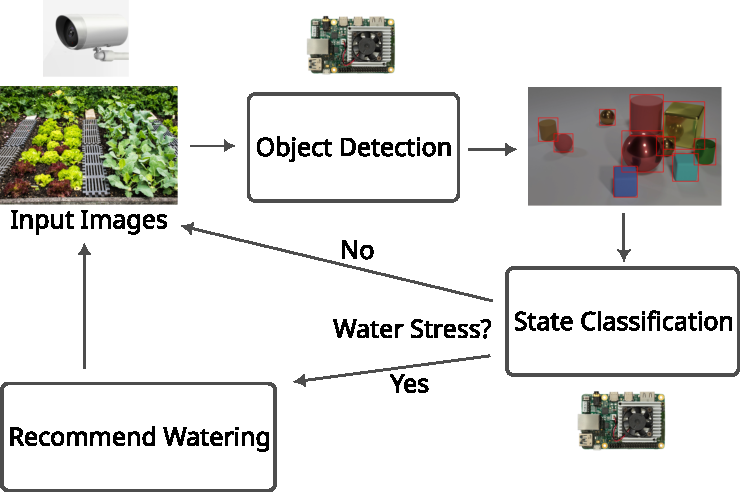
\includegraphics[width=0.8\textwidth]{graphics/setup.pdf}
  \caption[Methodological approach for the prototype.]{Methodological
    approach for the prototype. The prototype will run in a loop which
    starts at the top left corner. First, the camera attached to the
    prototype takes images of plants. These images are passed to the
    models running on the prototype. The first model generates
    bounding boxes for all detected plants. The bounding boxes are
    used to cut out the individual plants and pass them to the state
    classifier in sequence. The classifier outputs a probability score
    indicating the amount of stress the plant is experiencing. After a
    set amount of time, the camera takes a picture again and the
    process continues indefinitely.}
  \label{fig:setup}
\end{figure}

Estimated 1 page for this section.

\section{Selected Methods}
\label{sec:selected-methods}

Estimated 7 pages for this section.

\subsection{You Only Look Once}
\label{sec:methods-detection}

Describe the inner workings of the YOLOv7 model structure and contrast
it with previous versions as well as other object detectors. What has
changed and how did these improvements manifest themselves? Reference
the original paper~\cite{wang2022} and papers of previous versions of
the same model (YOLOv5~\cite{jocher2022},
YOLOv4~\cite{bochkovskiy2020}).

Estimated 2 pages for this section.

\subsection{ResNet}
\label{sec:methods-classification}

Introduce the approach of the \emph{ResNet} networks which implement
residual connections to allow deeper layers. Describe the inner
workings of the ResNet model structure. Reference the original
paper~\cite{he2016}.

Estimated 2 pages for this section.

Early research \cite{bengio1994,glorot2010} already demonstrated that
the vanishing/exploding gradient problem with standard gradient
descent and random initialization adversely affects convergence during
training and results in worse performance than would be otherwise
achievable with the same architecture. If a neural network is trained
with gradient descent by the application of the chain rule
(backpropagation), weight updates are passed from the later layers
back through the network to the early layers. Unfortunately, with some
activation functions (notably $\tanh$), the gradient can be very small
and decreases exponentially the further it passes through the
network. The effect being that the early layers do not receive any
weight updates which can stop the learning process entirely.

There are multiple potential solutions to the vanishing gradient
problem. Different weight initialization schemes
\cite{glorot2010,sussillo2015} as well as batch normalization layers
\cite{ioffe2015} can help mitigate the problem. The most effective
solution yet, however, was proposed as \emph{residual connections} by
\textcite{he2016}. Instead of connecting each layer only to the
previous and next layer in a sequential way, the authors add the input
of the previous layer to the output of the next layer. This is
achieved through the aforementioned residual or skip connections (see
figure~\ref{fig:residual-connection}).

\begin{figure}
  \centering
  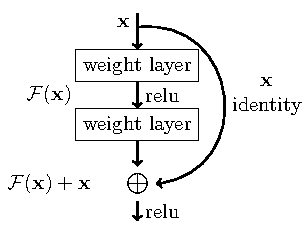
\includegraphics[width=0.35\textwidth]{graphics/residual-connection/res.pdf}
  \caption[Residual connection]{Residual connections: information from
    previous layers flows into subsequent layers before the activation
    function is applied. The symbol $\bigoplus$ represents simple
    element-wise addition. Figure redrawn from \textcite{he2016}.}
  \label{fig:residual-connection}
\end{figure}


\subsection{Data Augmentation}
\label{sec:methods-augmentation}

Go over the data augmentation methods which are used during training
for the object detector:
\begin{itemize}
\item HSV-hue
\item HSV-saturation
\item HSV-value
\item translation
\item scaling
\item inversion (left-right)
\item mosaic
\end{itemize}

Estimated 1 page for this section.

\subsection{Hyperparameter Optimization}
\label{sec:methods-hypopt}

Go into detail about the process used to optimize the detection and
classification models, what the training set looks like and how a
best-performing model was selected on the basis of the metrics.

Estimated 2 pages for this section.

\chapter{Prototype Implementation}
\label{chap:implementation}

\section{Object Detection}
\label{sec:development-detection}

Describe how the object detection model was trained and what the
training set looks like. Include a section on hyperparameter
optimization and go into detail about how the detector was optimized.

The object detection model was trained for 300 epochs on 79204 images
with 284130 ground truth labels. The weights from the best-performing
epoch were saved. The model's fitness for each epoch is calculated as
the weighted average of \textsf{mAP}@0.5 and \textsf{mAP}@0.5:0.95:

\begin{equation}
  \label{eq:fitness}
  f_{epoch} = 0.1 \cdot \mathsf{mAP}@0.5 + 0.9 \cdot \mathsf{mAP}@0.5\mathrm{:}0.95
\end{equation}

Figure~\ref{fig:fitness} shows the model's fitness over the training
period of 300 epochs. The gray vertical line indicates the maximum
fitness of 0.61 at epoch 133. The weights of that epoch were frozen to
be the final model parameters. Since the fitness metric assigns the
\textsf{mAP} at the higher range the overwhelming weight, the
\textsf{mAP}@0.5 starts to decrease after epoch 30, but the
\textsf{mAP}@0.5:0.95 picks up the slack until the maximum fitness at
epoch 133. This is an indication that the model achieves good
performance early on and continues to gain higher confidence values
until performance deteriorates due to overfitting.

\begin{figure}
  \centering
  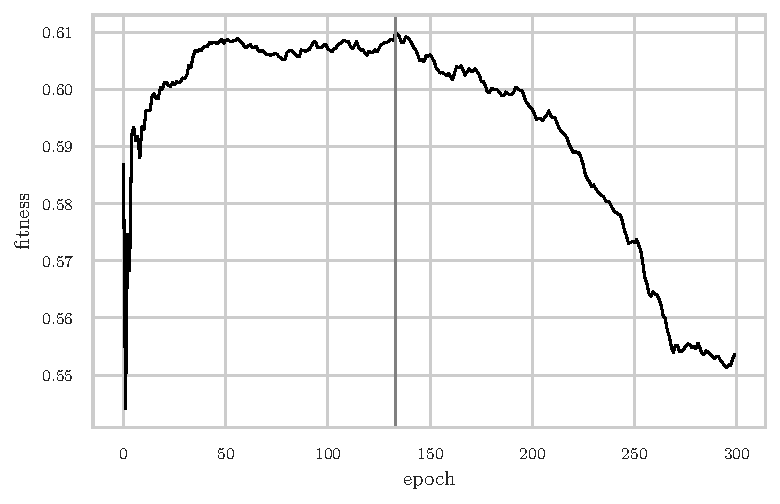
\includegraphics{graphics/model_fitness.pdf}
  \caption[Object detection fitness per epoch.]{Object detection model
    fitness for each epoch calculated as in
    equation~\ref{eq:fitness}. The vertical gray line at 133 marks the
    epoch with the highest fitness.}
  \label{fig:fitness}
\end{figure}

Overall precision and recall per epoch are shown in
figure~\ref{fig:prec-rec}. The values indicate that neither precision
nor recall change materially during training. In fact, precision
starts to decrease from the beginning, while recall experiences a
barely noticeable increase. Taken together with the box and object
loss from figure~\ref{fig:box-obj-loss}, we speculate that the
pre-trained model already generalizes well to plant detection because
one of the categories in the COCO~\cite{lin2015} dataset is
\emph{potted plant}. Any further training solely impacts the
confidence of detection, but does not lead to higher detection
rates. This conclusion is supported by the increasing
\textsf{mAP}@0.5:0.95 until epoch 133.

\begin{figure}
  \centering
  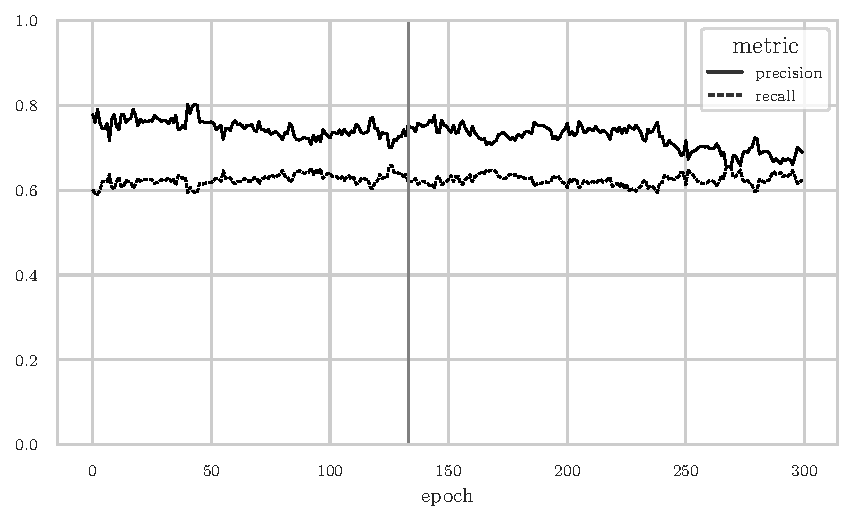
\includegraphics{graphics/precision_recall.pdf}
  \caption[Object detection precision and recall during
  training.]{Overall precision and recall during training for each
    epoch. The vertical gray line at 133 marks the epoch with the
    highest fitness.}
  \label{fig:prec-rec}
\end{figure}

Further culprits for the flat precision and recall values may be found
in bad ground truth data. The labels from the \gls{oid} are sometimes not
fine-grained enough. Images which contain multiple individual—often
overlapping—plants are labeled with one large bounding box instead of
multiple smaller ones. The model recognizes the individual plants and
returns tighter bounding boxes even if that is not what is specified
in the ground truth. Therefore, it is prudent to limit the training
phase to relatively few epochs in order to not penalize the more
accurate detections of the model. The smaller bounding boxes make more
sense considering the fact that the cutout is passed to the classifier
in a later stage. Smaller bounding boxes help the classifier to only
focus on one plant at a time and to not get distracted by multiple
plants in potentially different stages of wilting.

The box loss decreases slightly during training which indicates that
the bounding boxes become tighter around objects of interest. With
increasing training time, however, the object loss increases,
indicating that less and less plants are present in the predicted
bounding boxes. It is likely that overfitting is a cause for the
increasing object loss from epoch 40 onward. Since the best weights as
measured by fitness are found at epoch 133 and the object loss
accelerates from that point, epoch 133 is probably the correct cutoff
before overfitting occurs.

\begin{figure}
  \centering
  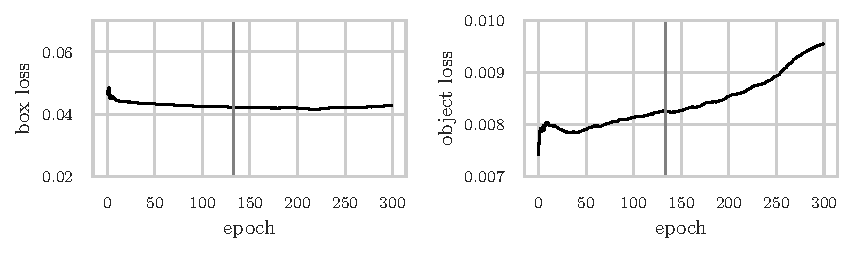
\includegraphics{graphics/val_box_obj_loss.pdf}
  \caption[Object detection box and object loss.]{Box and object loss
    measured against the validation set of 3091 images and 4092 ground
    truth labels. The class loss is omitted because there is only one
    class in the dataset and the loss is therefore always zero.}
  \label{fig:box-obj-loss}
\end{figure}

Estimated 2 pages for this section.

\section{Classification}
\label{sec:development-classification}

Describe how the classification model was trained and what the
training set looks like. Include a subsection hyperparameter
optimization and go into detail about how the classifier was
optimized.

The dataset was split 85/15 into training and validation sets. The
images in the training set were augmented with a random crop to arrive
at the expected image dimensions of 224 pixels. Additionally, the
training images were modified with a random horizontal flip to
increase the variation in the set and to train a rotation invariant
classifier. All images, regardless of their membership in the training
or validation set, were normalized with the mean and standard
deviation of the ImageNet~\cite{deng2009} dataset, which the original
\gls{resnet} model was pre-trained with. Training was done for 50
epochs and the best-performing model as measured by validation
accuracy was selected as the final version.

Figure~\ref{fig:classifier-training-metrics} shows accuracy and loss
on the training and validation sets. There is a clear upwards trend
until epoch 20 when validation accuracy and loss stabilize at around
0.84 and 0.3, respectively. The quick convergence and resistance to
overfitting can be attributed to the model already having robust
feature extraction capabilities.

\begin{figure}
  \centering
  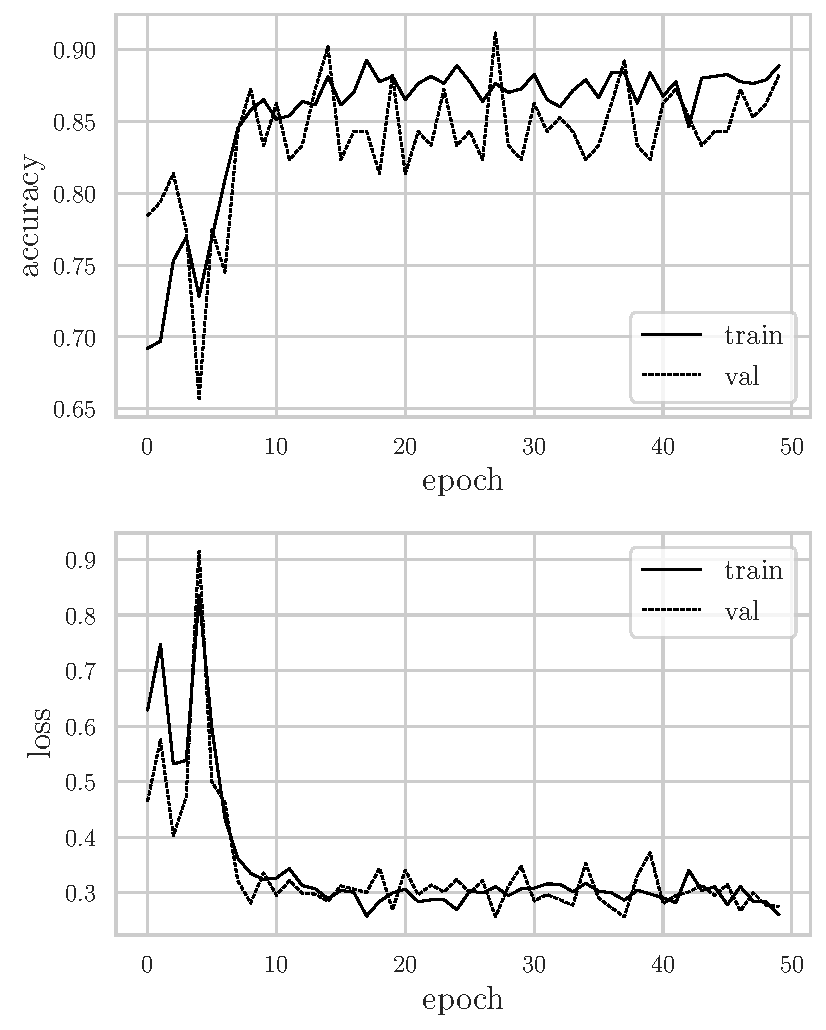
\includegraphics{graphics/classifier-metrics.pdf}
  \caption[Classifier accuracy and loss during training.]{Accuracy and
    loss during training of the classifier. The model converges
    quickly, but additional epochs do not cause validation loss to
    increase, which would indicate overfitting. The maximum validation
    accuracy of 0.9118 is achieved at epoch 27.}
  \label{fig:classifier-training-metrics}
\end{figure}

Estimated 2 pages for this section.

\section{Deployment}

Describe the Jetson Nano, how the model is deployed to the device and
how it reports its results (REST API).

Estimated 2 pages for this section.

\chapter{Evaluation}
\label{chap:evaluation}

The following sections contain a detailed evaluation of the model in
various scenarios. First, we present metrics from the training phases
of the constituent models. Second, we employ methods from the field of
\gls{xai} such as \gls{grad-cam} to get a better understanding of the
models' abstractions. Finally, we turn to the models' aggregate
performance on the test set.

\section{Methodology}
\label{sec:methodology}

Go over the evaluation methodology by explaining the test datasets,
where they come from, and how they're structured. Explain how the
testing phase was done and which metrics are employed to compare the
models to the SOTA.

Estimated 2 pages for this section.

\section{Results}
\label{sec:results}

Systematically go over the results from the testing phase(s), show the
plots and metrics, and explain what they contain. 

Estimated 4 pages for this section.

\subsection{Object Detection}
\label{ssec:yolo-eval}

The following parapraph should probably go into
section~\ref{sec:development-detection}.

The object detection model was pre-trained on the COCO~\cite{lin2015}
dataset and fine-tuned with data from the \gls{oid}
\cite{kuznetsova2020} in its sixth version. Since the full \gls{oid}
dataset contains considerably more classes and samples than would be
feasibly trainable on a small cluster of \glspl{gpu}, only images from
the two classes \emph{Plant} and \emph{Houseplant} have been
downloaded. The samples from the Houseplant class are merged into the
Plant class because the distinction between the two is not necessary
for our model. Furthermore, the \gls{oid} contains not only bounding
box annotations for object detection tasks, but also instance
segmentations, classification labels and more. These are not needed
for our purposes and are omitted as well. In total, the dataset
consists of 91479 images with a roughly 85/5/10 split for training,
validation and testing, respectively.

\subsubsection{Test Phase}
\label{sssec:yolo-test}

Of the 91479 images around 10\% were used for the test phase. These
images contain a total of 12238 ground truth
labels. Table~\ref{tab:yolo-metrics} shows precision, recall and the
harmonic mean of both (F1-score). The results indicate that the model
errs on the side of sensitivity because recall is higher than
precision. Although some detections are not labeled as plants in the
dataset, if there is a labeled plant in the ground truth data, the
chance is high that it will be detected. This behavior is in line with
how the model's detections are handled in practice. The detections are
drawn on the original image and the user is able to check the bounding
boxes visually. If there are wrong detections, the user can ignore
them and focus on the relevant ones instead. A higher recall will thus
serve the user's needs better than a high precision.

\begin{table}[h]
  \centering
  \begin{tabular}{lrrrr}
    \toprule
    {} &  Precision &    Recall &  F1-score &  Support \\
    \midrule
    Plant        &   0.547571 &  0.737866 &  0.628633 &  12238.0 \\
    \bottomrule
  \end{tabular}
  \caption{Precision, recall and F1-score for the object detection model.}
  \label{tab:yolo-metrics}
\end{table}

Figure~\ref{fig:yolo-ap} shows the \gls{ap} for the \gls{iou}
thresholds of 0.5 and 0.95. Predicted bounding boxes with an \gls{iou}
of less than 0.5 are not taken into account for the precision and
recall values of table~\ref{tab:yolo-metrics}. The lower the detection
threshold, the more plants are detected. Conversely, a higher
detection threshold leaves potential plants undetected. The
precision-recall curves confirm this behavior because the area under
the curve for the threshold of 0.5 is higher than for the threshold of
0.95 ($0.66$ versus $0.41$). These values are combined in COCO's
\cite{lin2015} main evaluation metric which is the \gls{ap} averaged
across the \gls{iou} thresholds from 0.5 to 0.95 in 0.05 steps. This
value is then averaged across all classes and called \gls{map}. The
object detection model achieves a state-of-the-art \gls{map} of 0.5727
for the \emph{Plant} class.

\begin{figure}
  \centering
  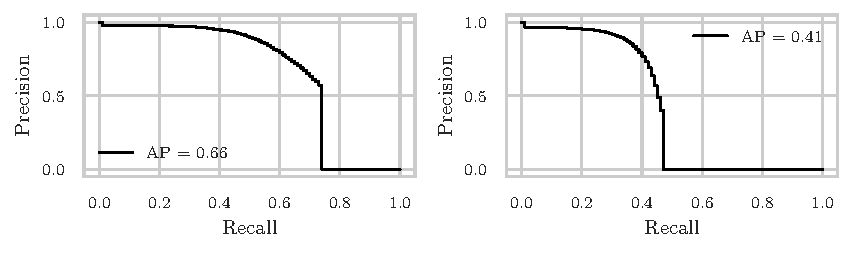
\includegraphics{graphics/APpt5-pt95.pdf}
  \caption[Object detection AP@0.5 and AP@0.95.]{Precision-recall
    curves for \gls{iou} thresholds of 0.5 and 0.95. The \gls{ap} of a
    specific threshold is defined as the area under the
    precision-recall curve of that threshold. The \gls{map} across
    \gls{iou} thresholds from 0.5 to 0.95 in 0.05 steps
    \textsf{mAP}@0.5:0.95 is 0.5727.}
  \label{fig:yolo-ap}
\end{figure}

\subsubsection{Hyperparameter Optimization}
\label{sssec:yolo-hyp-opt}

This section should be moved to the hyperparameter optimization
section in the development chapter
(section~\ref{sec:development-detection}).

To further improve the object detection performance, we perform
hyper-parameter optimization using a genetic algorithm. Evolution of
the hyper-parameters starts from the initial 30 default values
provided by the authors of YOLO. Of those 30 values, 26 are allowed to
mutate. During each generation, there is an 80\% chance that a
mutation occurs with a variance of 0.04. To determine which generation
should be the parent of the new mutation, all previous generations are
ordered by fitness in decreasing order. At most five top generations
are selected and one of them is chosen at random. Better generations
have a higher chance of being selected as the selection is weighted by
fitness. The parameters of that chosen generation are then mutated
with the aforementioned probability and variance. Each generation is
trained for three epochs and the fitness of the best epoch is
recorded.

In total, we ran 87 iterations of which the 34\textsuperscript{th}
generation provides the best fitness of 0.6076. Due to time
constraints, it was not possible to train each generation for more
epochs or to run more iterations in total. We assume that the
performance of the first few epochs is a reasonable proxy for model
performance overall. The optimized version of the object detection
model is then trained for 70 epochs using the parameters of the
34\textsuperscript{th} generation.

\begin{figure}
  \centering
  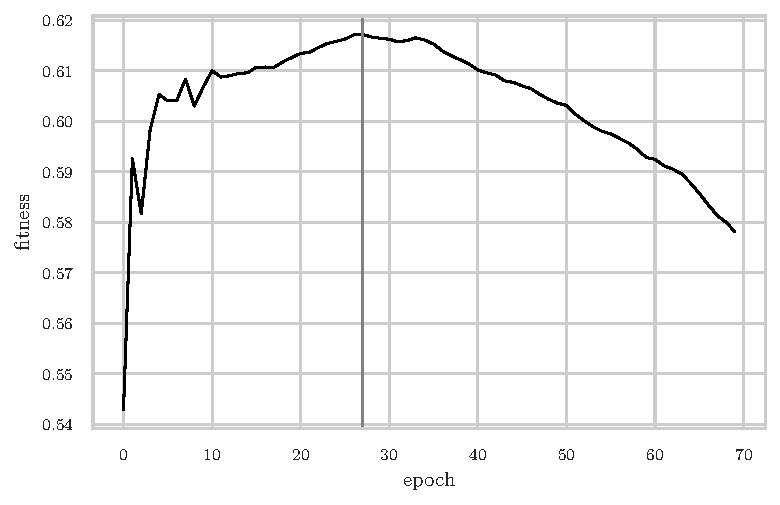
\includegraphics{graphics/model_fitness_final.pdf}
  \caption[Optimized object detection fitness per epoch.]{Object
    detection model fitness for each epoch calculated as in
    equation~\ref{eq:fitness}. The vertical gray line at 27 marks the
    epoch with the highest fitness of 0.6172.}
  \label{fig:hyp-opt-fitness}
\end{figure}

Figure~\ref{fig:hyp-opt-fitness} shows the model's fitness during
training for each epoch. After the highest fitness of 0.6172 at epoch
27, the performance quickly declines and shows that further training
would likely not yield improved results. The model converges to its
highest fitness much earlier than the non-optimized version, which
indicates that the adjusted parameters provide a better starting point
in general. Furthermore, the maximum fitness is 0.74\% higher than in
the non-optimized version.

\begin{figure}
  \centering
  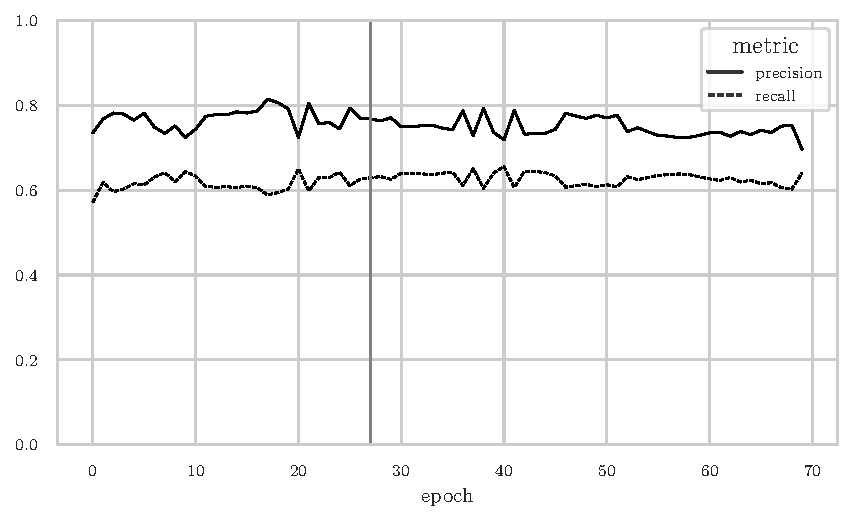
\includegraphics{graphics/precision_recall_final.pdf}
  \caption[Hyper-parameter optimized object detection precision and
  recall during training.]{Overall precision and recall during
    training for each epoch of the optimized model. The vertical gray
    line at 27 marks the epoch with the highest fitness.}
  \label{fig:hyp-opt-prec-rec}
\end{figure}

Figure~\ref{fig:hyp-opt-prec-rec} shows precision and recall for the
optimized model during training. Similarly to the non-optimized model
from figure~\ref{fig:prec-rec}, both metrics do not change materially
during training. Precision is slightly higher than in the
non-optimized version and recall hovers at the same levels.

\begin{figure}
  \centering
  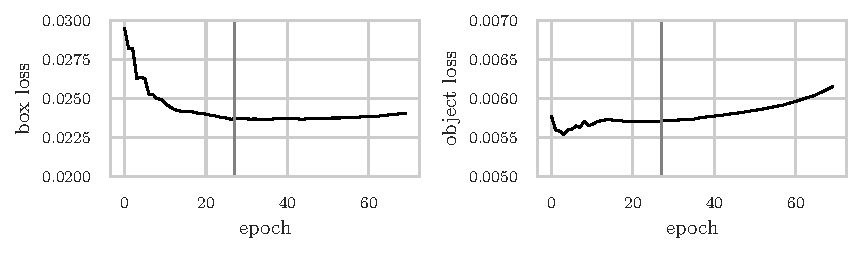
\includegraphics{graphics/val_box_obj_loss_final.pdf}
  \caption[Hyper-parameter optimized object detection box and object
  loss.]{Box and object loss measured against the validation set of
    3091 images and 4092 ground truth labels. The class loss is
    omitted because there is only one class in the dataset and the
    loss is therefore always zero.}
  \label{fig:hyp-opt-box-obj-loss}
\end{figure}

The box and object loss during training is pictured in
figure~\ref{fig:hyp-opt-box-obj-loss}. Both losses start from a lower
level which suggests that the initial optimized parameters allow the
model to converge quicker. The object loss exhibits a similar slope to
the non-optimized model in figure~\ref{fig:box-obj-loss}. The vertical
gray line again marks epoch 27 with the highest fitness. The box loss
reaches its lower limit at that point and the object loss starts to
increase again after epoch 27.

\begin{table}[h]
  \centering
  \begin{tabular}{lrrrr}
    \toprule
    {} &  Precision &    Recall &  F1-score &  Support \\
    \midrule
    Plant        &   0.633358 &  0.702811 &  0.666279 &  12238.0 \\
    \bottomrule
  \end{tabular}
  \caption{Precision, recall and F1-score for the optimized object
    detection model.}
  \label{tab:yolo-metrics-hyp}
\end{table}

Turning to the evaluation of the optimized model on the test dataset,
table~\ref{tab:yolo-metrics-hyp} shows precision, recall and the
F1-score for the optimized model. Comparing these metrics with the
non-optimized version from table~\ref{tab:yolo-metrics}, precision is
significantly higher by more than 8.5\%. Recall, however, is 3.5\%
lower. The F1-score is higher by more than 3.7\% which indicates that
the optimized model is better overall despite the lower recall. We
feel that the lower recall value is a suitable trade off for the
substantially higher precision considering that the non-optimized
model's precision is quite low at 0.55.

The precision-recall curves in figure~\ref{fig:yolo-ap-hyp} for the
optimized model show that the model draws looser bounding boxes than
the optimized model. The \gls{ap} for both \gls{iou} thresholds of 0.5
and 0.95 is lower indicating worse performance. It is likely that more
iterations during evolution would help increase the \gls{ap} values as
well. Even though the precision and recall values from
table~\ref{tab:yolo-metrics-hyp} are better, the \textsf{mAP}@0.5:0.95
is lower by 1.8\%.

\begin{figure}
  \centering
  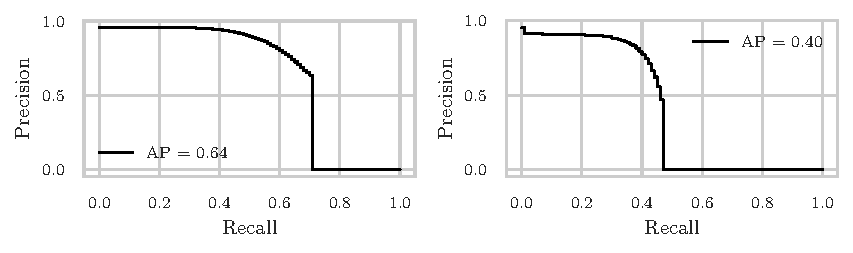
\includegraphics{graphics/APpt5-pt95-final.pdf}
  \caption[Hyper-parameter optimized object detection AP@0.5 and
  AP@0.95.]{Precision-recall curves for \gls{iou} thresholds of 0.5
    and 0.95. The \gls{ap} of a specific threshold is defined as the
    area under the precision-recall curve of that threshold. The
    \gls{map} across \gls{iou} thresholds from 0.5 to 0.95 in 0.05
    steps \textsf{mAP}@0.5:0.95 is 0.5546.}
  \label{fig:yolo-ap-hyp}
\end{figure}

\subsection{Classification}
\label{ssec:classifier-eval}

The classifier receives cutouts from the object detection model and
determines whether the image shows a stressed plant or not. To achieve
this goal, we trained a \gls{resnet} \cite{he2016} on a dataset of 452
images of healthy and 452 stressed plants. We chose the \gls{resnet}
architecture due to its popularity and ease of implementation as well
as its consistently high performance on various classification
tasks. While its classification speed in comparison with networks
optimized for mobile and edge devices (e.g. MobileNet) is
significantly lower, the deeper structure and the additional
parameters are necessary for the fairly complex task at
hand. Furthermore, the generous time budget for object detection
\emph{and} classification allows for more accurate results at the
expense of speed. The architecture allows for multiple different
structures, depending on the amount of layers. The smallest one has 18
and the largest 152 layers with 34, 50 and 101 in-between. The larger
networks have better accuracy in general, but come with trade-offs
regarding training and inference time as well as required space. The
50 layer architecture (\gls{resnet}50) is adequate for our use case.

\subsubsection{Hyperparameter Optimization}
\label{sssec:classifier-hyp-opt}

This section should be moved to the hyperparameter optimization
section in the development chapter
(section~\ref{sec:development-classification}).

In order to improve the aforementioned accuracy values, we perform
hyper-parameter optimization across a wide range of
parameters. Table~\ref{tab:classifier-hyps} lists the hyper-parameters
and their possible values. Since the number of all combinations of
values is 11520 and each combination is trained for 10 epochs with a
training time of approximately six minutes per combination, exhausting
the search space would take 48 days. Due to time limitations, we have
chosen to not search exhaustively but to pick random combinations
instead. Random search works surprisingly well---especially compared to
grid search---in a number of domains, one of which is hyper-parameter
optimization~\cite{bergstra2012}.

\begin{table}[h]
  \centering
  \begin{tabular}{lr}
    \toprule
    Parameter &  Values \\
    \midrule
    optimizer &	adam, sgd \\
    batch size & 4, 8, 16, 32, 64 \\
    learning rate & 0.0001, 0.0003, 0.001, 0.003, 0.01, 0.1 \\
    step size & 2, 3, 5, 7 \\
    gamma & 0.1, 0.5 \\
    beta one & 0.9, 0.99 \\
    beta two & 0.5, 0.9, 0.99, 0.999 \\
    eps & 0.00000001, 0.1, 1 \\
    \bottomrule
  \end{tabular}
  \caption{Hyper-parameters and their possible values during
    optimization.}
  \label{tab:classifier-hyps}
\end{table}

The random search was run for 138 iterations which equates to a 75\%
probability that the best solution lies within 1\% of the theoretical
maximum~\eqref{eq:opt-prob}. Figure~\ref{fig:classifier-hyp-results}
shows three of the eight parameters and their impact on a high
F1-score. \gls{sgd} has less variation in its results than
Adam~\cite{kingma2017} and manages to provide eight out of the ten
best results. The number of epochs to train for was chosen based on
the observation that almost all configurations converge well before
reaching the tenth epoch. The assumption that a training run with ten
epochs provides a good proxy for final performance is supported by the
quick convergence of validation accuracy and loss in
figure~\ref{fig:classifier-training-metrics}.

\begin{equation}\label{eq:opt-prob}
  1 - (1 - 0.01)^{138} \approx 0.75
\end{equation}

\begin{figure}
  \centering
  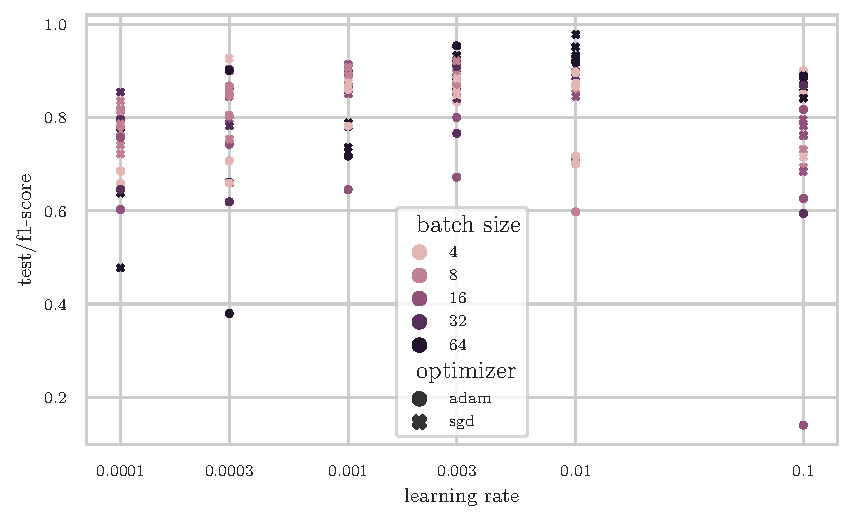
\includegraphics{graphics/classifier-hyp-metrics.pdf}
  \caption[Classifier hyper-parameter optimization results.]{This
    figure shows three of the eight hyper-parameters and their
    performance measured by the F1-score during 138
    trials. Differently colored markers show the batch size with
    darker colors representing a larger batch size. The type of marker
    (circle or cross) shows which optimizer was used. The x-axis shows
    the learning rate on a logarithmic scale. In general, a learning
    rate between 0.003 and 0.01 results in more robust and better
    F1-scores. Larger batch sizes more often lead to better
    performance as well. As for the type of optimizer, \gls{sgd}
    produced the best iteration with an F1-score of 0.9783. Adam tends
    to require more customization of its parameters than \gls{sgd} to
    achieve good results.}
  \label{fig:classifier-hyp-results}
\end{figure}

Table~\ref{tab:classifier-final-hyps} lists the final hyper-parameters
which were chosen to train the improved model. In order to confirm
that the model does not suffer from overfitting or is a product of
chance due to a coincidentally advantageous train/test split, we
perform stratified $10$-fold cross validation on the dataset. Each
fold contains 90\% training and 10\% test data and was trained for 25
epochs. Figure~\ref{fig:classifier-hyp-roc} shows the performance of
the epoch with the highest F1-score of each fold as measured against
the test split. The mean \gls{roc} curve provides a robust metric for
a classifier's performance because it averages out the variability of
the evaluation. Each fold manages to achieve at least an \gls{auc} of
0.94, while the best fold reaches 0.98. The mean \gls{roc} has an
\gls{auc} of 0.96 with a standard deviation of 0.02. These results
indicate that the model is accurately predicting the correct class and
is robust against variations in the training set.

\begin{table}
  \centering
  \begin{tabular}{cccc}
    \toprule
    Optimizer &  Batch Size & Learning Rate & Step Size \\
    \midrule
    \gls{sgd} & 64 & 0.01 & 5\\
    \bottomrule
  \end{tabular}
  \caption[Hyper-parameters for the optimized classifier.]{Chosen
    hyper-parameters for the final, improved model. The difference to
    the parameters listed in Table~\ref{tab:classifier-hyps} comes as
    a result of choosing \gls{sgd} over Adam. The missing four
    parameters are only required for Adam and not \gls{sgd}.}
  \label{tab:classifier-final-hyps}
\end{table}

\begin{figure}
  \centering
  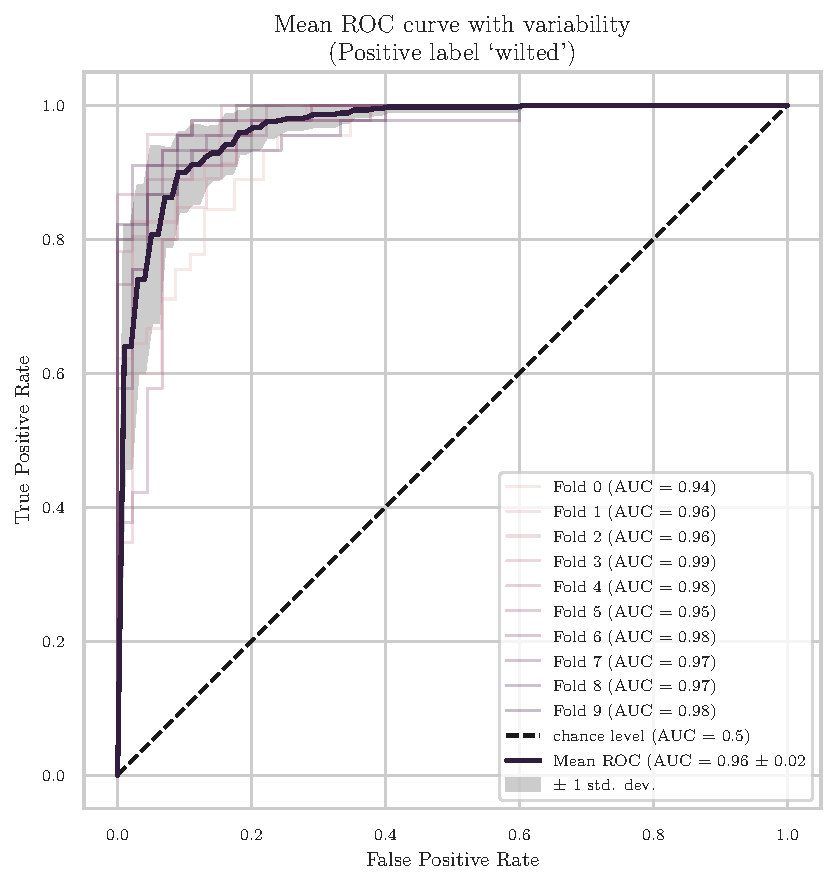
\includegraphics{graphics/classifier-hyp-folds-roc.pdf}
  \caption[Mean \gls{roc} and variability of hyper-parameter-optimized
  model.]{This plot shows the \gls{roc} curve for the epoch with the
    highest F1-score of each fold as well as the \gls{auc}. To get a
    less variable performance metric of the classifier, the mean
    \gls{roc} curve is shown as a thick line and the variability is
    shown in gray. The overall mean \gls{auc} is 0.96 with a standard
    deviation of 0.02. The best-performing fold reaches an \gls{auc}
    of 0.99 and the worst an \gls{auc} of 0.94. The black dashed line
    indicates the performance of a classifier which picks classes at
    random ($\mathrm{\gls{auc}} = 0.5$). The shapes of the \gls{roc}
    curves show that the classifier performs well and is robust
    against variations in the training set.}
  \label{fig:classifier-hyp-roc}
\end{figure}

The classifier shows good performance so far, but care has to be taken
to not overfit the model to the training set. Comparing the F1-score
during training with the F1-score during testing gives insight into
when the model tries to increase its performance during training at
the expense of generalizability. Figure~\ref{fig:classifier-hyp-folds}
shows the F1-scores of each epoch and fold. The classifier converges
quickly to 1 for the training set at which point it experiences a
slight drop in generalizability. Training the model for at most five
epochs is sufficient because there are generally no improvements
afterwards. The best-performing epoch for each fold is between the
second and fourth epoch which is just before the model achieves an
F1-score of 1 on the training set.

\begin{figure}
  \centering
  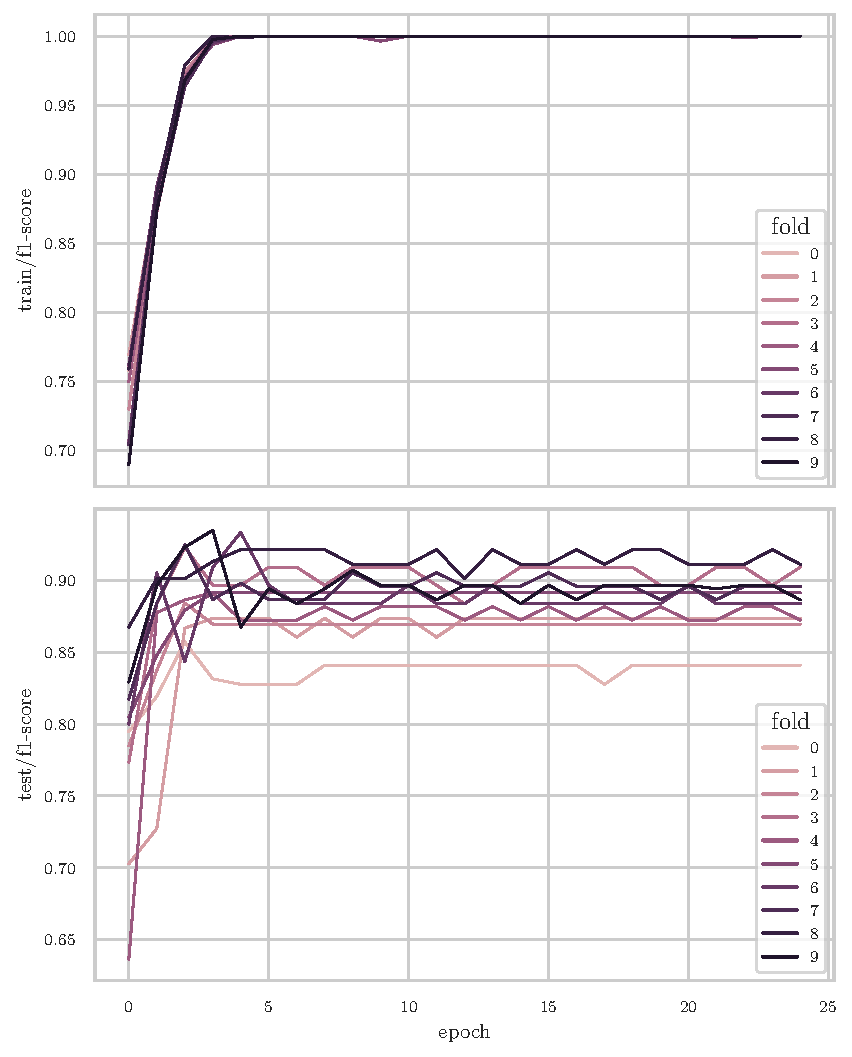
\includegraphics[width=.9\textwidth]{graphics/classifier-hyp-folds-f1.pdf}
  \caption[F1-score of stratified $10$-fold cross validation.]{These
    plots show the F1-score during training as well as testing for
    each of the folds. The classifier converges to 1 by the third
    epoch during the training phase, which might indicate
    overfitting. However, the performance during testing increases
    until epoch three in most cases and then stabilizes at
    approximately 2-3\% lower than the best epoch. We believe that the
    third, or in some cases fourth, epoch is detrimental to
    performance and results in overfitting, because the model achieves
    an F1-score of 1 for the training set, but that gain does not
    transfer to the test set. Early stopping during training
    alleviates this problem.}
  \label{fig:classifier-hyp-folds}
\end{figure}


\subsubsection{Class Activation Maps}
\label{sssec:classifier-cam}

Neural networks are notorious for their black-box behavior, where it
is possible to observe the inputs and the corresponding outputs, but
the stage in-between stays hidden from view. Models are continuously
developed and deployed to aid in human decision-making and sometimes
supplant it. It is, therefore, crucial to obtain some amount of
interpretability of what the model does \emph{inside} to be able to
explain why a decision was made in a certain way. The research field
of \gls{xai} gained significance during the last few years because of
the development of new methods to peek inside these black boxes.

One such method, \gls{cam}~\cite{zhou2015}, is a popular tool to
produce visual explanations for decisions made by
\glspl{cnn}. Convolutional layers essentially function as object
detectors as long as no fully-connected layers perform the
classification. This ability to localize regions of interest, which
play a significant role in the type of class the model predicts, can
be retained until the last layer and used to generate activation maps
for the predictions.

A more recent approach to generating a \gls{cam} via gradients is
proposed by~\textcite{selvaraju2020}. Their \gls{grad-cam} approach
works by computing the gradient of the feature maps of the last
convolutional layer with respect to the specified class. The last
layer is chosen because the authors find that ``[…]  Grad-CAM maps
become progressively worse as we move to earlier convolutional layers
as they have smaller receptive fields and only focus on less semantic
local features.''~\cite[p.5]{selvaraju2020}

Turning to our classifier, figure~\ref{fig:classifier-cam} shows the
\glspl{cam} for \emph{healthy} and \emph{stressed}. While the regions
of interest for the \emph{healthy} class lie on the healthy plant, the
\emph{stressed} plant is barely considered and mostly rendered as
background information (blue). Conversely, when asked to explain the
inputs to the \emph{stressed} classification, the regions of interest
predominantly stay on the thirsty as opposed to the healthy plant. In
fact, the large hanging leaves play a significant role in determining
the class the image belongs to. This is an additional data point
confirming that the model focuses on the semantically meaningful parts
of the image during classification.

\begin{figure}
  \centering
  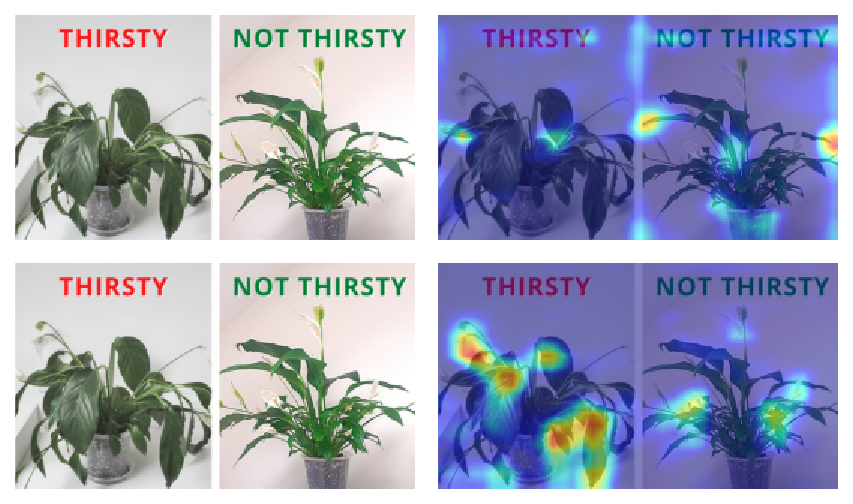
\includegraphics{graphics/classifier-cam.pdf}
  \caption[Classifier \glspl{cam}.]{The top left image shows the
    original image of the same plant in a stressed (left) and healthy
    (right) state. In the top right image, the \gls{cam} for the class
    \emph{healthy} is laid over the original image. The classifier
    draws its conclusion mainly from the healthy plant, which is
    indicated by the red hot spots around the tips of the plant. The
    bottom right image shows the \gls{cam} for the \emph{stressed}
    class. The classifier focuses on the hanging leaves of the thirsty
    plant. The image was classified as \emph{stressed} with a
    confidence of 70\%.}
  \label{fig:classifier-cam}
\end{figure}


\subsection{Aggregate Model}
\label{ssec:aggregate-model}

In this section we turn to the evaluation of the aggregate model. We
have confirmed the performance of the constituent models: the object
detection and the classification model. It remains to evaluate the
complete pipeline from gathering detections of potential plants in an
image and forwarding them to the classifier to obtaining the results
as either healthy or stressed with their associated confidence scores.

The test set contains 640 images which were obtained from a google
search using the terms \emph{thirsty plant}, \emph{wilted plant} and
\emph{stressed plant}. Images which clearly show one or multiple
plants with some amount of visible stress were added to the
dataset. Care was taken to include plants with various degrees of
stress and in various locations and lighting conditions. The search
not only provided images of stressed plants, but also of healthy
plants due to articles, which describe how to care for plants, having
a banner image of healthy plants. The dataset is biased towards potted
plants which are commonly put on display in western
households. Furthermore, many plants, such as succulents, are sought
after for home environments because of their ease of maintenance. Due
to their inclusion in the dataset and how they exhibit water stress,
the test set nevertheless contains a wide variety of scenarios.

After collecting the images, the aggregate model was run on them to
obtain initial bounding boxes and classifications for ground truth
labeling. Letting the model do the work beforehand and then correcting
the labels allowed to include more images in the test set because they
could be labeled more easily. Additionally, going over the detections
and classifications provided a comprehensive view on how the models
work and what their weaknesses and strengths are. After the labels
have been corrected, the ground truth of the test set contains 766
bounding boxes of healthy plants and 494 of stressed plants.

\subsection{Non-optimized Model}
\label{ssec:model-non-optimized}

\begin{table}
  \centering
  \begin{tabular}{lrrrr}
    \toprule
    {} &  precision &  recall &  f1-score &  support \\
    \midrule
    Healthy      &      0.665 &   0.554 &     0.604 &    766 \\
    Stressed     &      0.639 &   0.502 &     0.562 &    494 \\
    micro avg    &      0.655 &   0.533 &     0.588 &   1260 \\
    macro avg    &      0.652 &   0.528 &     0.583 &   1260 \\
    weighted avg &      0.655 &   0.533 &     0.588 &   1260 \\
    \bottomrule
  \end{tabular}
  \caption{Precision, recall and F1-score for the aggregate model.}
  \label{tab:model-metrics}
\end{table}

Table~\ref{tab:model-metrics} shows precision, recall and the F1-score
for both classes \emph{Healthy} and \emph{Stressed}. Precision is
higher than recall for both classes and the F1-score is at
0.59. Unfortunately, these values do not take the accuracy of bounding
boxes into account and thus have only limited expressive power.

Figure~\ref{fig:aggregate-ap} shows the precision and recall curves
for both classes at different \gls{iou} thresholds. The left plot
shows the \gls{ap} for each class at the threshold of 0.5 and the
right one at 0.95. The \gls{map} is 0.3581 and calculated across all
classes as the median of the \gls{iou} thresholds from 0.5 to 0.95 in
0.05 steps. The cliffs at around 0.6 (left) and 0.3 (right) happen at
a detection threshold of 0.5. The classifier's last layer is a softmax
layer which necessarily transforms the input into a probability of
showing either a healthy or stressed plant. If the probability of an
image showing a healthy plant is below 0.5, it is no longer classified
as healthy but as stressed. The threshold for discriminating the two
classes lies at the 0.5 value and is therefore the cutoff for either
class.

\begin{figure}
  \centering
  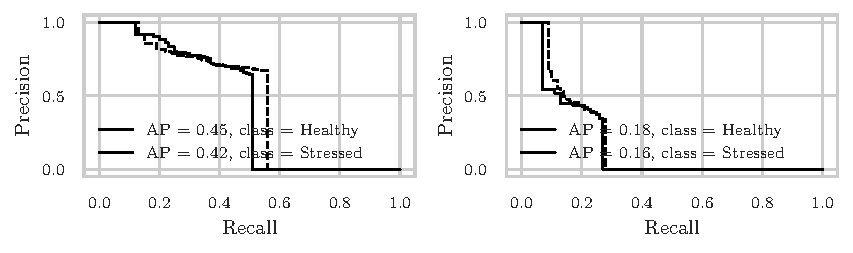
\includegraphics{graphics/APmodel-model-optimized-relabeled.pdf}
  \caption[Aggregate model AP@0.5 and AP@0.95.]{Precision-recall
    curves for \gls{iou} thresholds of 0.5 and 0.95. The \gls{ap} of a
    specific threshold is defined as the area under the
    precision-recall curve of that threshold. The \gls{map} across
    \gls{iou} thresholds from 0.5 to 0.95 in 0.05 steps
    \textsf{mAP}@0.5:0.95 is 0.3581.}
  \label{fig:aggregate-ap}
\end{figure}

\subsection{Optimized Model}
\label{ssec:model-optimized}

So far the metrics shown in table~\ref{tab:model-metrics} are obtained
with the non-optimized versions of both the object detection and
classification model. Hyper-parameter optimization of the classifier
led to significant model improvements, while the object detector has
improved precision but lower recall and slightly lower \gls{map}
values. To evaluate the final aggregate model which consists of the
individual optimized models, we run the same test described in
section~\ref{ssec:aggregate-model}.

\begin{table}
  \centering
  \begin{tabular}{lrrrr}
    \toprule
    {} &  precision &  recall &  f1-score &  support \\
    \midrule
    Healthy      &      0.711 &   0.555 &     0.623 &    766 \\
    Stressed     &      0.570 &   0.623 &     0.596 &    494 \\
    micro avg    &      0.644 &   0.582 &     0.611 &   1260 \\
    macro avg    &      0.641 &   0.589 &     0.609 &   1260 \\
    weighted avg &      0.656 &   0.582 &     0.612 &   1260 \\
    \bottomrule
  \end{tabular}
  \caption{Precision, recall and F1-score for the optimized aggregate
    model.}
  \label{tab:model-metrics-hyp}
\end{table}

Table~\ref{tab:model-metrics-hyp} shows precision, recall and F1-score
for the optimized model on the same test dataset of 640 images. All of
the metrics are better for the optimized model. In particular,
precision for the healthy class could be improved significantly while
recall remains at the same level. This results in a better F1-score
for the healthy class. Precision for the stressed class is lower with
the optimized model, but recall is significantly higher (0.502
vs. 0.623). The higher recall results in a 3\% gain for the F1-score
in the stressed class. Overall, precision is the same but recall has
improved significantly, which also results in a noticeable improvement
for the average F1-score across both classes.

\begin{figure}
  \centering
  \includegraphics{graphics/APModel-model-original-relabeled.pdf}
  \caption[Optimized aggregate model AP@0.5 and
  AP@0.95.]{Precision-recall curves for \gls{iou} thresholds of 0.5
    and 0.95. The \gls{ap} of a specific threshold is defined as the
    area under the precision-recall curve of that threshold. The
    \gls{map} across \gls{iou} thresholds from 0.5 to 0.95 in 0.05
    steps \textsf{mAP}@0.5:0.95 is 0.3838.}
  \label{fig:aggregate-ap-hyp}
\end{figure}

Figure~\ref{fig:aggregate-ap-hyp} confirms the performance increase of
the optimized model established in
table~\ref{tab:model-metrics-hyp}. The \textsf{mAP}@0.5 is higher for
both classes, indicating that the model better detects plants in
general. The \textsf{mAP}@0.95 is slightly lower for the healthy
class, which means that the confidence for the healthy class is
slightly lower compared to the non-optimized model. The result is that
more plants are correctly detected and classified overall, but the
confidence scores tend to be lower with the optimized model. The
\textsf{mAP}@0.5:0.95 could be improved by about 0.025.

\section{Discussion}
\label{sec:discussion}

Pull out discussion parts from current results chapter
(~\ref{sec:results}) and add a section about achievement of the aim
of the work discussed in motivation and problem statement section
(~\ref{sec:methods}).

Estimated 2 pages for this chapter.

\chapter{Conclusion}
\label{chap:conclusion}

Conclude the thesis with a short recap of the results and the
discussion. Establish whether the research questions from
section~\ref{sec:methods} can be answered successfully.

Estimated 2 pages for this chapter.

\section{Future Work}
\label{sec:future-work}

Suggest further research directions regarding the approach. Give an
outlook on further possibilities in this research field with respect
to object detection and plant classification.

Estimated 1 page for this section

\backmatter

% Use an optional list of figures.
\listoffigures % Starred version, i.e., \listoffigures*, removes the toc entry.

% Use an optional list of tables.
\cleardoublepage % Start list of tables on the next empty right hand page.
\listoftables % Starred version, i.e., \listoftables*, removes the toc entry.

% Use an optional list of algorithms.
\listofalgorithms
\addcontentsline{toc}{chapter}{List of Algorithms}

% Add an index.
\printindex

% Add a glossary.
\printglossaries

% Add a bibliography.
%\bibliographystyle{alpha}
\printbibliography

\end{document}
%%% Local Variables:
%%% mode: latex
%%% TeX-master: "thesis"
%%% TeX-master: t
%%% TeX-master: t
%%% TeX-master: t
%%% TeX-master: t
%%% TeX-master: t
%%% TeX-master: t
%%% TeX-master: t
%%% TeX-master: t
%%% TeX-master: t
%%% TeX-master: t
%%% TeX-master: t
%%% TeX-master: t
%%% TeX-master: t
%%% TeX-master: t
%%% TeX-master: t
%%% End:
